% Options for packages loaded elsewhere
\PassOptionsToPackage{unicode}{hyperref}
\PassOptionsToPackage{hyphens}{url}
\PassOptionsToPackage{dvipsnames,svgnames,x11names}{xcolor}
%
\documentclass[
  ignorenonframetext,
]{beamer}
\usepackage{pgfpages}
\setbeamertemplate{caption}[numbered]
\setbeamertemplate{caption label separator}{: }
\setbeamercolor{caption name}{fg=normal text.fg}
\beamertemplatenavigationsymbolsempty
% Prevent slide breaks in the middle of a paragraph
\widowpenalties 1 10000
\raggedbottom
\setbeamertemplate{part page}{
  \centering
  \begin{beamercolorbox}[sep=16pt,center]{part title}
    \usebeamerfont{part title}\insertpart\par
  \end{beamercolorbox}
}
\setbeamertemplate{section page}{
  \centering
  \begin{beamercolorbox}[sep=12pt,center]{part title}
    \usebeamerfont{section title}\insertsection\par
  \end{beamercolorbox}
}
\setbeamertemplate{subsection page}{
  \centering
  \begin{beamercolorbox}[sep=8pt,center]{part title}
    \usebeamerfont{subsection title}\insertsubsection\par
  \end{beamercolorbox}
}
\AtBeginPart{
  \frame{\partpage}
}
\AtBeginSection{
  \ifbibliography
  \else
    \frame{\sectionpage}
  \fi
}
\AtBeginSubsection{
  \frame{\subsectionpage}
}
\usepackage{amsmath,amssymb}
\usepackage{iftex}
\ifPDFTeX
  \usepackage[T1]{fontenc}
  \usepackage[utf8]{inputenc}
  \usepackage{textcomp} % provide euro and other symbols
\else % if luatex or xetex
  \usepackage{unicode-math} % this also loads fontspec
  \defaultfontfeatures{Scale=MatchLowercase}
  \defaultfontfeatures[\rmfamily]{Ligatures=TeX,Scale=1}
\fi
\usepackage{lmodern}
\ifPDFTeX\else
  % xetex/luatex font selection
\fi
% Use upquote if available, for straight quotes in verbatim environments
\IfFileExists{upquote.sty}{\usepackage{upquote}}{}
\IfFileExists{microtype.sty}{% use microtype if available
  \usepackage[]{microtype}
  \UseMicrotypeSet[protrusion]{basicmath} % disable protrusion for tt fonts
}{}
\makeatletter
\@ifundefined{KOMAClassName}{% if non-KOMA class
  \IfFileExists{parskip.sty}{%
    \usepackage{parskip}
  }{% else
    \setlength{\parindent}{0pt}
    \setlength{\parskip}{6pt plus 2pt minus 1pt}}
}{% if KOMA class
  \KOMAoptions{parskip=half}}
\makeatother
\usepackage{xcolor}
\newif\ifbibliography
\setlength{\emergencystretch}{3em} % prevent overfull lines
\providecommand{\tightlist}{%
  \setlength{\itemsep}{0pt}\setlength{\parskip}{0pt}}
\setcounter{secnumdepth}{-\maxdimen} % remove section numbering
%\ProvidesPackage{config/presento}

\mode<presentation>

% removing navigation symbols
\setbeamertemplate{navigation symbols}{}

% packages
\usepackage{xcolor}
\usepackage{fontspec}
\usepackage{setspace}
\usepackage{tikz}
\usepackage{multicol}
\usepackage{multirow}
\usepackage{philex}

% colors
\definecolor{colorblack}{HTML}{000000} % for note
\definecolor{colorgreen}{HTML}{009933} % for code
\definecolor{colorwhite}{HTML}{FFFFFF} % background
\definecolor{colorblue}{HTML}{0099CC} % blue
\definecolor{colorbig}{HTML}{1f77b4} % for note
\definecolor{colormedium}{HTML}{ff7f0e} % for note
\definecolor{colorsmall}{HTML}{2ca02c} % for note


% font sizes
\newcommand{\fontsizeone}{1em}
\newcommand{\fontsizetwo}{0.85em}
\newcommand{\fontsizethree}{1em}
% line spaces
\newcommand{\linespaceone}{1}

% font families
\newfontfamily{\inconsolatafont}[Path=fonts/]{brill}

% beamer template changes
\setbeamertemplate{frametitle}{
 \vspace{0.40em}
 \noindent
 \hspace{-1.22em}
 \tikz[overlay,remember picture,baseline=0.3em]{\fill[fill= colorblue]  (-0.3,0.05) rectangle (0,0.9); }\color{colorblue}~~\insertframetitle%
}

\setmainfont[Ligatures=TeX,Path=fonts/,
						BoldFont=brillb,
						ItalicFont=brilli,
						BoldItalicFont=brillbi,
						SmallCapsFont=brill]{brill}
\setsansfont[Ligatures=TeX,Path=fonts/,
						BoldFont=brillb,
						ItalicFont=brilli,
						BoldItalicFont=brillbi,
						SmallCapsFont=brill]{brill}
\setmonofont[Scale=0.7, Path=fonts/]{iosevka-regular}

% frame counter
\newcounter{totalfr}
\setbeamertemplate{footline}{
  \ifnum\inserttotalframenumber=1
    \setcounter{totalfr}{2}
  \else
     \setcounter{totalfr}{\inserttotalframenumber}
  \fi
  \hfill{
    \tikz{
      \filldraw[fill=colorblue!80, draw=colorblue!80]  (0,0) -- (0.2,0) arc (0:{\value{framenumber}*(360/(\value{totalfr}))}:0.2) -- (0,0); 
      \node at (0,0) {\normalsize \color{colorblack}\tiny{\insertframenumber}};
    }
  }
  \hspace{2em}
  \vspace*{1em}
}

% custom commands
\newcommand{\hugetext}[1]{
  {
  \begin{spacing}{\linespaceone}
   \fontsize{\fontsizeone}{\fontsizeone}{ #1}
  \end{spacing}
  }
}

\newcommand{\largetext}[1]{
 {\fontsize{\fontsizetwo}{\fontsizeone}\selectfont{#1}}
}

\newcommand{\setnote}[1]{
 {\fontsize{\fontsizethree}{\fontsizeone}\selectfont\color{colorblack}{#1}}
}

\newcommand{\framecard}[2][colorblue]{
  {\setbeamercolor{background canvas}{bg=#1}
    \begin{frame}[plain]
    \vfill
    \begin{center}
     {#2}
    \end{center}
    \vfill
    \end{frame}
  }
}
\newcommand{\framepic}[3][1]{
  {
    \usebackgroundtemplate{%
    \tikz[overlay,remember picture] \node[opacity=#1, at=(current page.center)] {
      \includegraphics[width=\paperwidth]{#2}};
    }
    \begin{frame}
    #3
    \end{frame}
  }
}

\setbeamercolor{background canvas}{bg=colorwhite}
\setbeamercolor{normal text}{fg=colorblack}
\setbeamercolor{title}{fg=colorblue}
\setbeamercolor{subtitle}{fg=colorblue}
\setbeamercolor{author}{fg=colorblack}
\setbeamercolor{alerted text}{fg=colorblue}

\defbeamertemplate*{title page}{customized}[1][]
{
  \vfill
  {\usebeamercolor[fg]{title}\hugetext{\inserttitle}}
  {\usebeamerfont{subtitle}\usebeamercolor[fg]{subtitle}\largetext{\insertsubtitle}\par}
  \vfill
  {\usebeamercolor[fg]{author}\largetext{\insertauthor}}\\
  {\setnote{\insertinstitute}\par}
  \vfill
  {\setnote{\insertdate}\par}
  \vfill
}

\usepackage{natbib}
\bibpunct[: ]{(}{)}{;}{a}{}{,}

\setbeamertemplate{itemize items}{\color{colorblue}$\bullet$}
\setbeamertemplate{enumerate items}{\color{colorblue}$\theenumi$.}
\setbeamertemplate{frametitle continuation}{}
\setbeamercolor{block title}{fg=colorblue,bg=white} 

\usepackage{hyperref}
\hypersetup{linkcolor=colorblue, colorlinks=true}

\AtBeginSection[]
{
  \begin{frame}
    \frametitle{План презентации}
    \tableofcontents[currentsection]
  \end{frame}
}

\setbeamertemplate{caption}{\raggedright\insertcaption\par}
\ifLuaTeX
  \usepackage{selnolig}  % disable illegal ligatures
\fi
\usepackage[]{natbib}
\bibliographystyle{plainnat}
\IfFileExists{bookmark.sty}{\usepackage{bookmark}}{\usepackage{hyperref}}
\IfFileExists{xurl.sty}{\usepackage{xurl}}{} % add URL line breaks if available
\urlstyle{same}
\hypersetup{
  pdftitle={Опыт зеркальной лаборатории},
  colorlinks=true,
  linkcolor={Maroon},
  filecolor={Maroon},
  citecolor={colorblue},
  urlcolor={colorblue},
  pdfcreator={LaTeX via pandoc}}

\title{Опыт зеркальной лаборатории}
\author{Г. А. Мороз\\
\strut \\
\small  Международная лаборатория языковой конвергенции (НИУ ВШЭ,
Москва)}
\date{14 декабря 2023}

\begin{document}
\frame{\titlepage}

\hypertarget{ux43e-ux43cux435ux436ux434ux443ux43dux430ux440ux43eux434ux43dux43eux439-ux43bux430ux431ux43eux440ux430ux442ux43eux440ux438ux438-ux44fux437ux44bux43aux43eux432ux43eux439-ux43aux43eux43dux432ux435ux440ux433ux435ux43dux446ux438ux438}{%
\section{О международной лаборатории языковой
конвергенции}\label{ux43e-ux43cux435ux436ux434ux443ux43dux430ux440ux43eux434ux43dux43eux439-ux43bux430ux431ux43eux440ux430ux442ux43eux440ux438ux438-ux44fux437ux44bux43aux43eux432ux43eux439-ux43aux43eux43dux432ux435ux440ux433ux435ux43dux446ux438ux438}}

\begin{frame}{Международная лаборатория языковой конвергенции}
\protect\hypertarget{ux43cux435ux436ux434ux443ux43dux430ux440ux43eux434ux43dux430ux44f-ux43bux430ux431ux43eux440ux430ux442ux43eux440ux438ux44f-ux44fux437ux44bux43aux43eux432ux43eux439-ux43aux43eux43dux432ux435ux440ux433ux435ux43dux446ux438ux438}{}
\begin{itemize}
\tightlist
\item
  Открыта в 2017 году
\end{itemize}

\begin{figure}

{\centering 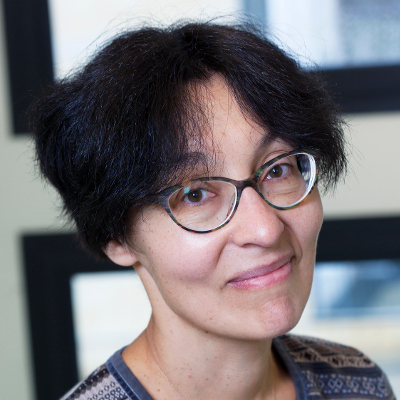
\includegraphics[width=0.4\linewidth]{images/01_dobrushina} 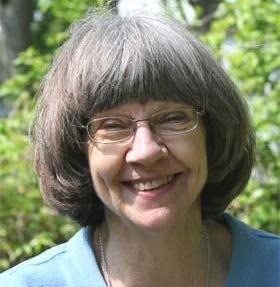
\includegraphics[width=0.4\linewidth]{images/02_nichols} 

}

\caption{Н. Р. Добрушина и Дж. Николс}\label{fig:unnamed-chunk-2}
\end{figure}

Оба исследователя специализируются на славянских языках и языках
Кавказа, а также лингвистической типологии
\end{frame}

\begin{frame}{Миссия}
\protect\hypertarget{ux43cux438ux441ux441ux438ux44f}{}
Исследование механизмов конвергентных процессов в истории языка, то есть
языковых ситуаций, при которых контакт между носителями разных языков
ведет к появлению у этих языков общих черт. В лаборатории
разрабатываются инструменты для выявления результатов таких процессов по
данным электронных корпусов устной речи и создаются каталоги таких
явлений на материале малых языков России.
\end{frame}

\begin{frame}{Ресурсы международной лаборатории языковой конвергенции}
\protect\hypertarget{ux440ux435ux441ux443ux440ux441ux44b-ux43cux435ux436ux434ux443ux43dux430ux440ux43eux434ux43dux43eux439-ux43bux430ux431ux43eux440ux430ux442ux43eux440ux438ux438-ux44fux437ux44bux43aux43eux432ux43eux439-ux43aux43eux43dux432ux435ux440ux433ux435ux43dux446ux438ux438}{}
\begin{itemize}
\tightlist
\item
  lingconlab.ru
\item
  22 устных корпуса диалектов русского языка
\item
  8 устных корпусов русского языка билингвов
\item
  10 корпусов малых языков
\item
  другие

  \begin{itemize}
  \tightlist
  \item
    словари (мегебский, рутульский, тукитинский, хваршинский,
    даргинский)
  \item
    Типологический атлас языков Дагестана
  \item
    Атлас многоязычия в Дагестане
  \item
    Атлас рутульских диалектов
  \item
    Корпус Просодии Русских Диалектов (ПРуД)
  \item
    \ldots{}
  \end{itemize}
\end{itemize}
\end{frame}

\begin{frame}{22 устных диалектных корпуса}
\protect\hypertarget{ux443ux441ux442ux43dux44bux445-ux434ux438ux430ux43bux435ux43aux442ux43dux44bux445-ux43aux43eux440ux43fux443ux441ux430}{}
\begin{center}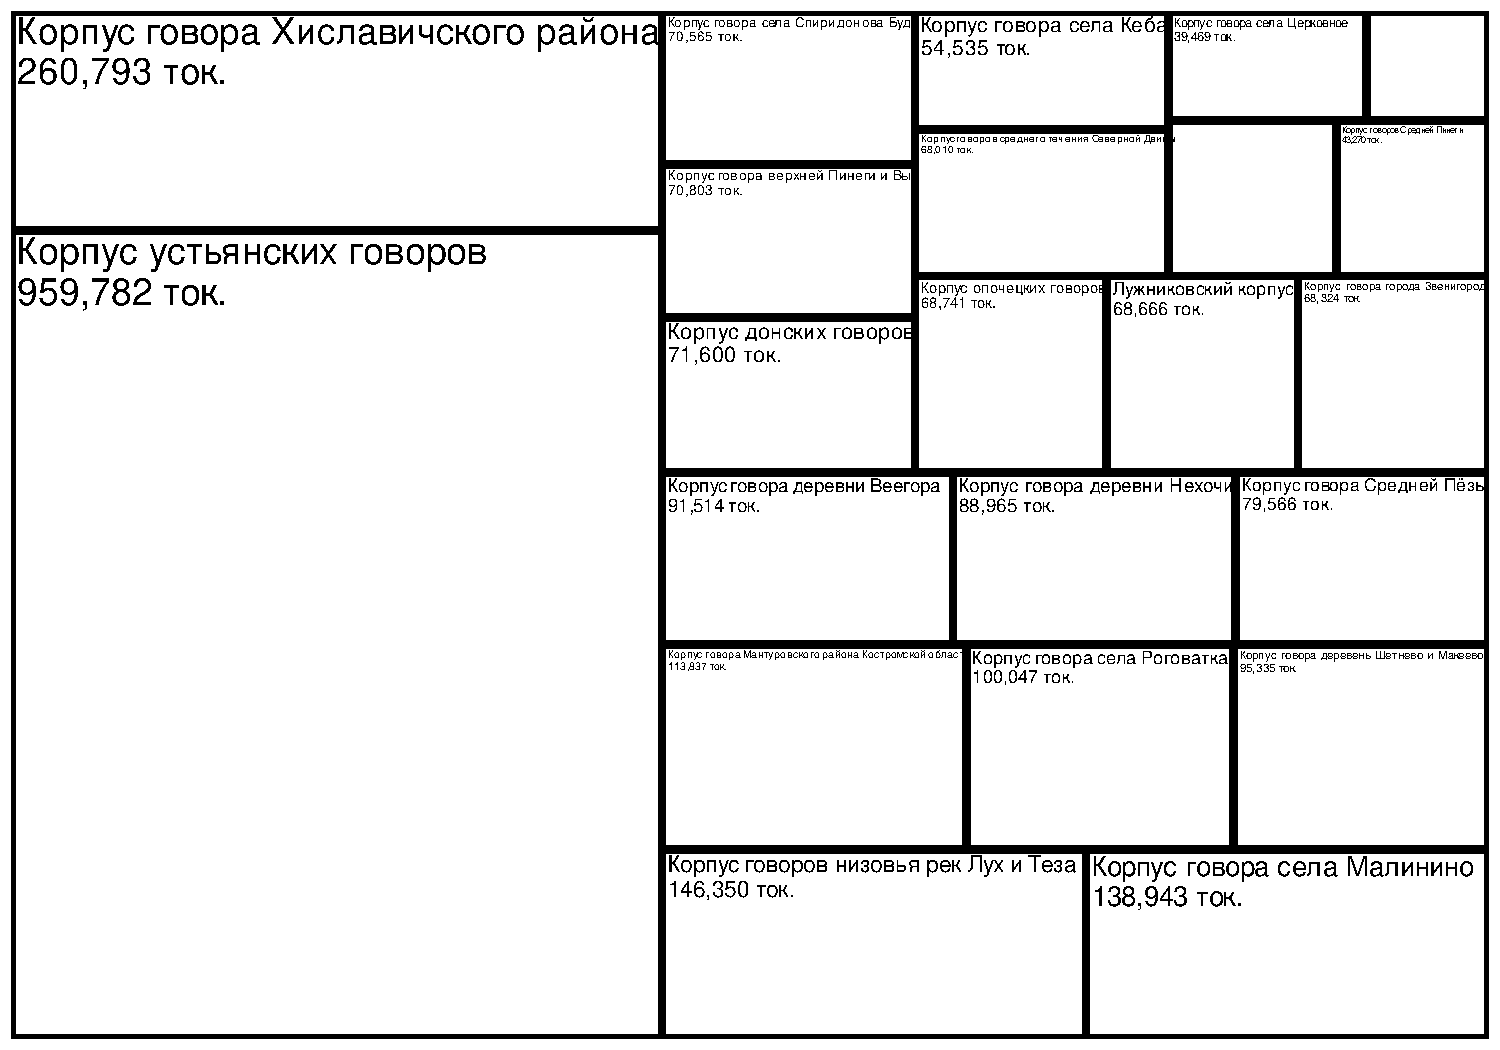
\includegraphics[width=0.99\linewidth]{2023.12.14_4nv_files/figure-beamer/unnamed-chunk-3-1} \end{center}
\end{frame}

\begin{frame}{22 устных диалектных корпуса}
\protect\hypertarget{ux443ux441ux442ux43dux44bux445-ux434ux438ux430ux43bux435ux43aux442ux43dux44bux445-ux43aux43eux440ux43fux443ux441ux430-1}{}
\begin{center}\includegraphics[width=0.71\linewidth]{images/01_dialects} \end{center}
\end{frame}

\begin{frame}{8 устных билингавльных корпусов}
\protect\hypertarget{ux443ux441ux442ux43dux44bux445-ux431ux438ux43bux438ux43dux433ux430ux432ux43bux44cux43dux44bux445-ux43aux43eux440ux43fux443ux441ux43eux432}{}
\begin{center}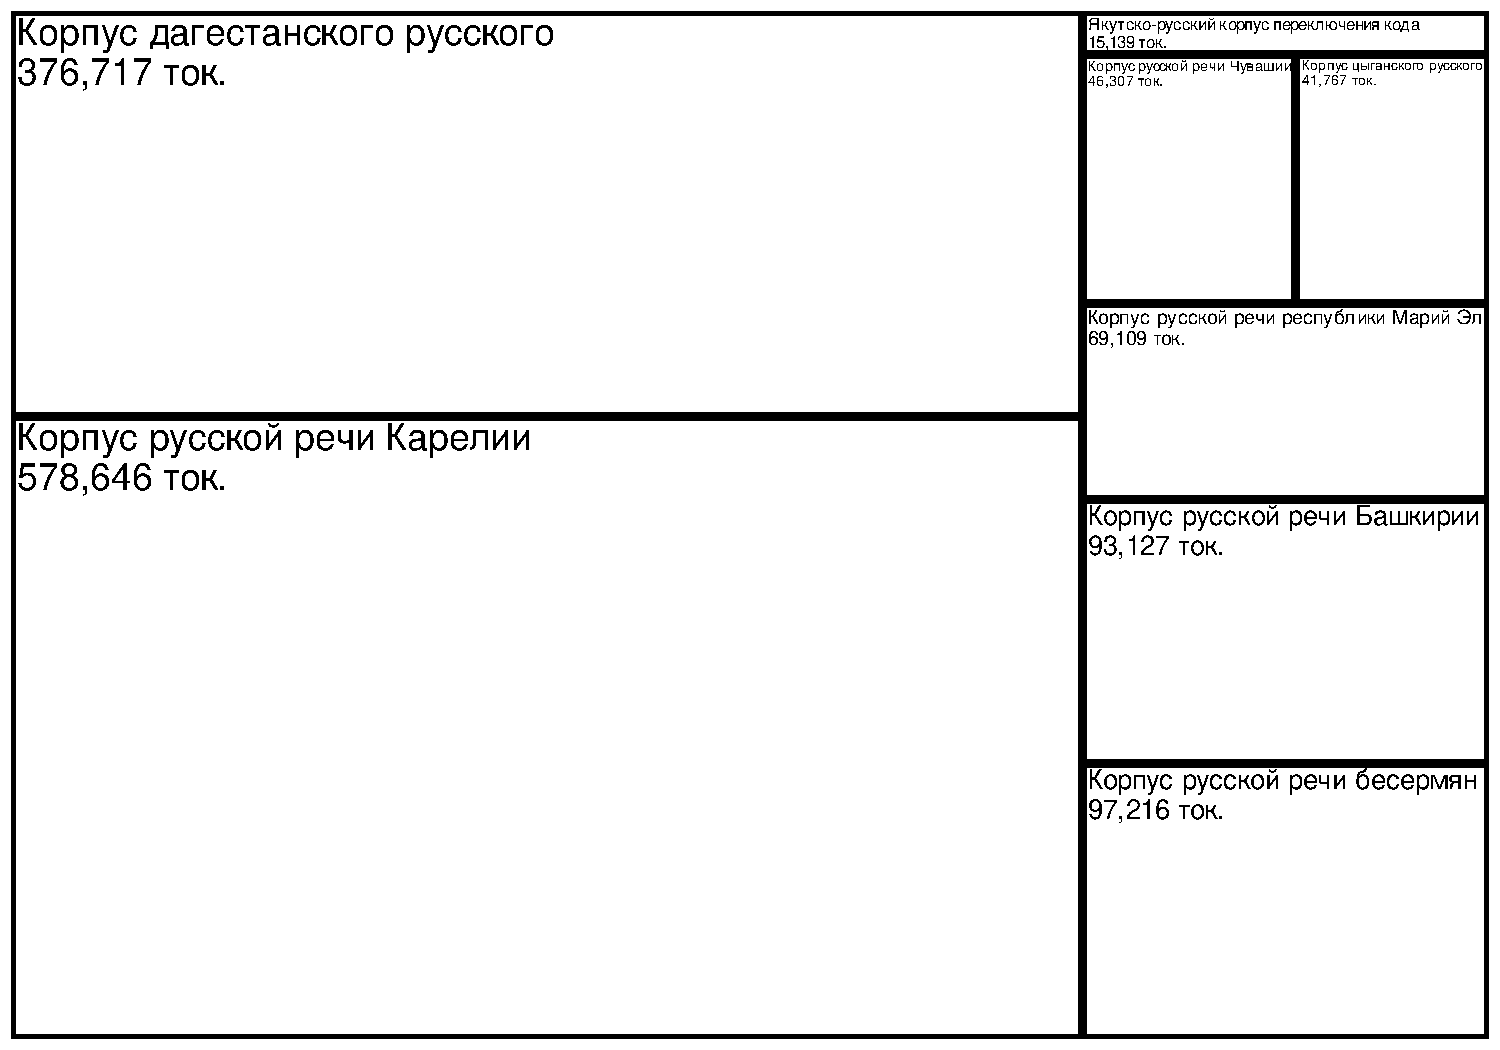
\includegraphics[width=0.99\linewidth]{2023.12.14_4nv_files/figure-beamer/unnamed-chunk-6-1} \end{center}
\end{frame}

\begin{frame}{8 устных билингавльных корпусов}
\protect\hypertarget{ux443ux441ux442ux43dux44bux445-ux431ux438ux43bux438ux43dux433ux430ux432ux43bux44cux43dux44bux445-ux43aux43eux440ux43fux443ux441ux43eux432-1}{}
\begin{center}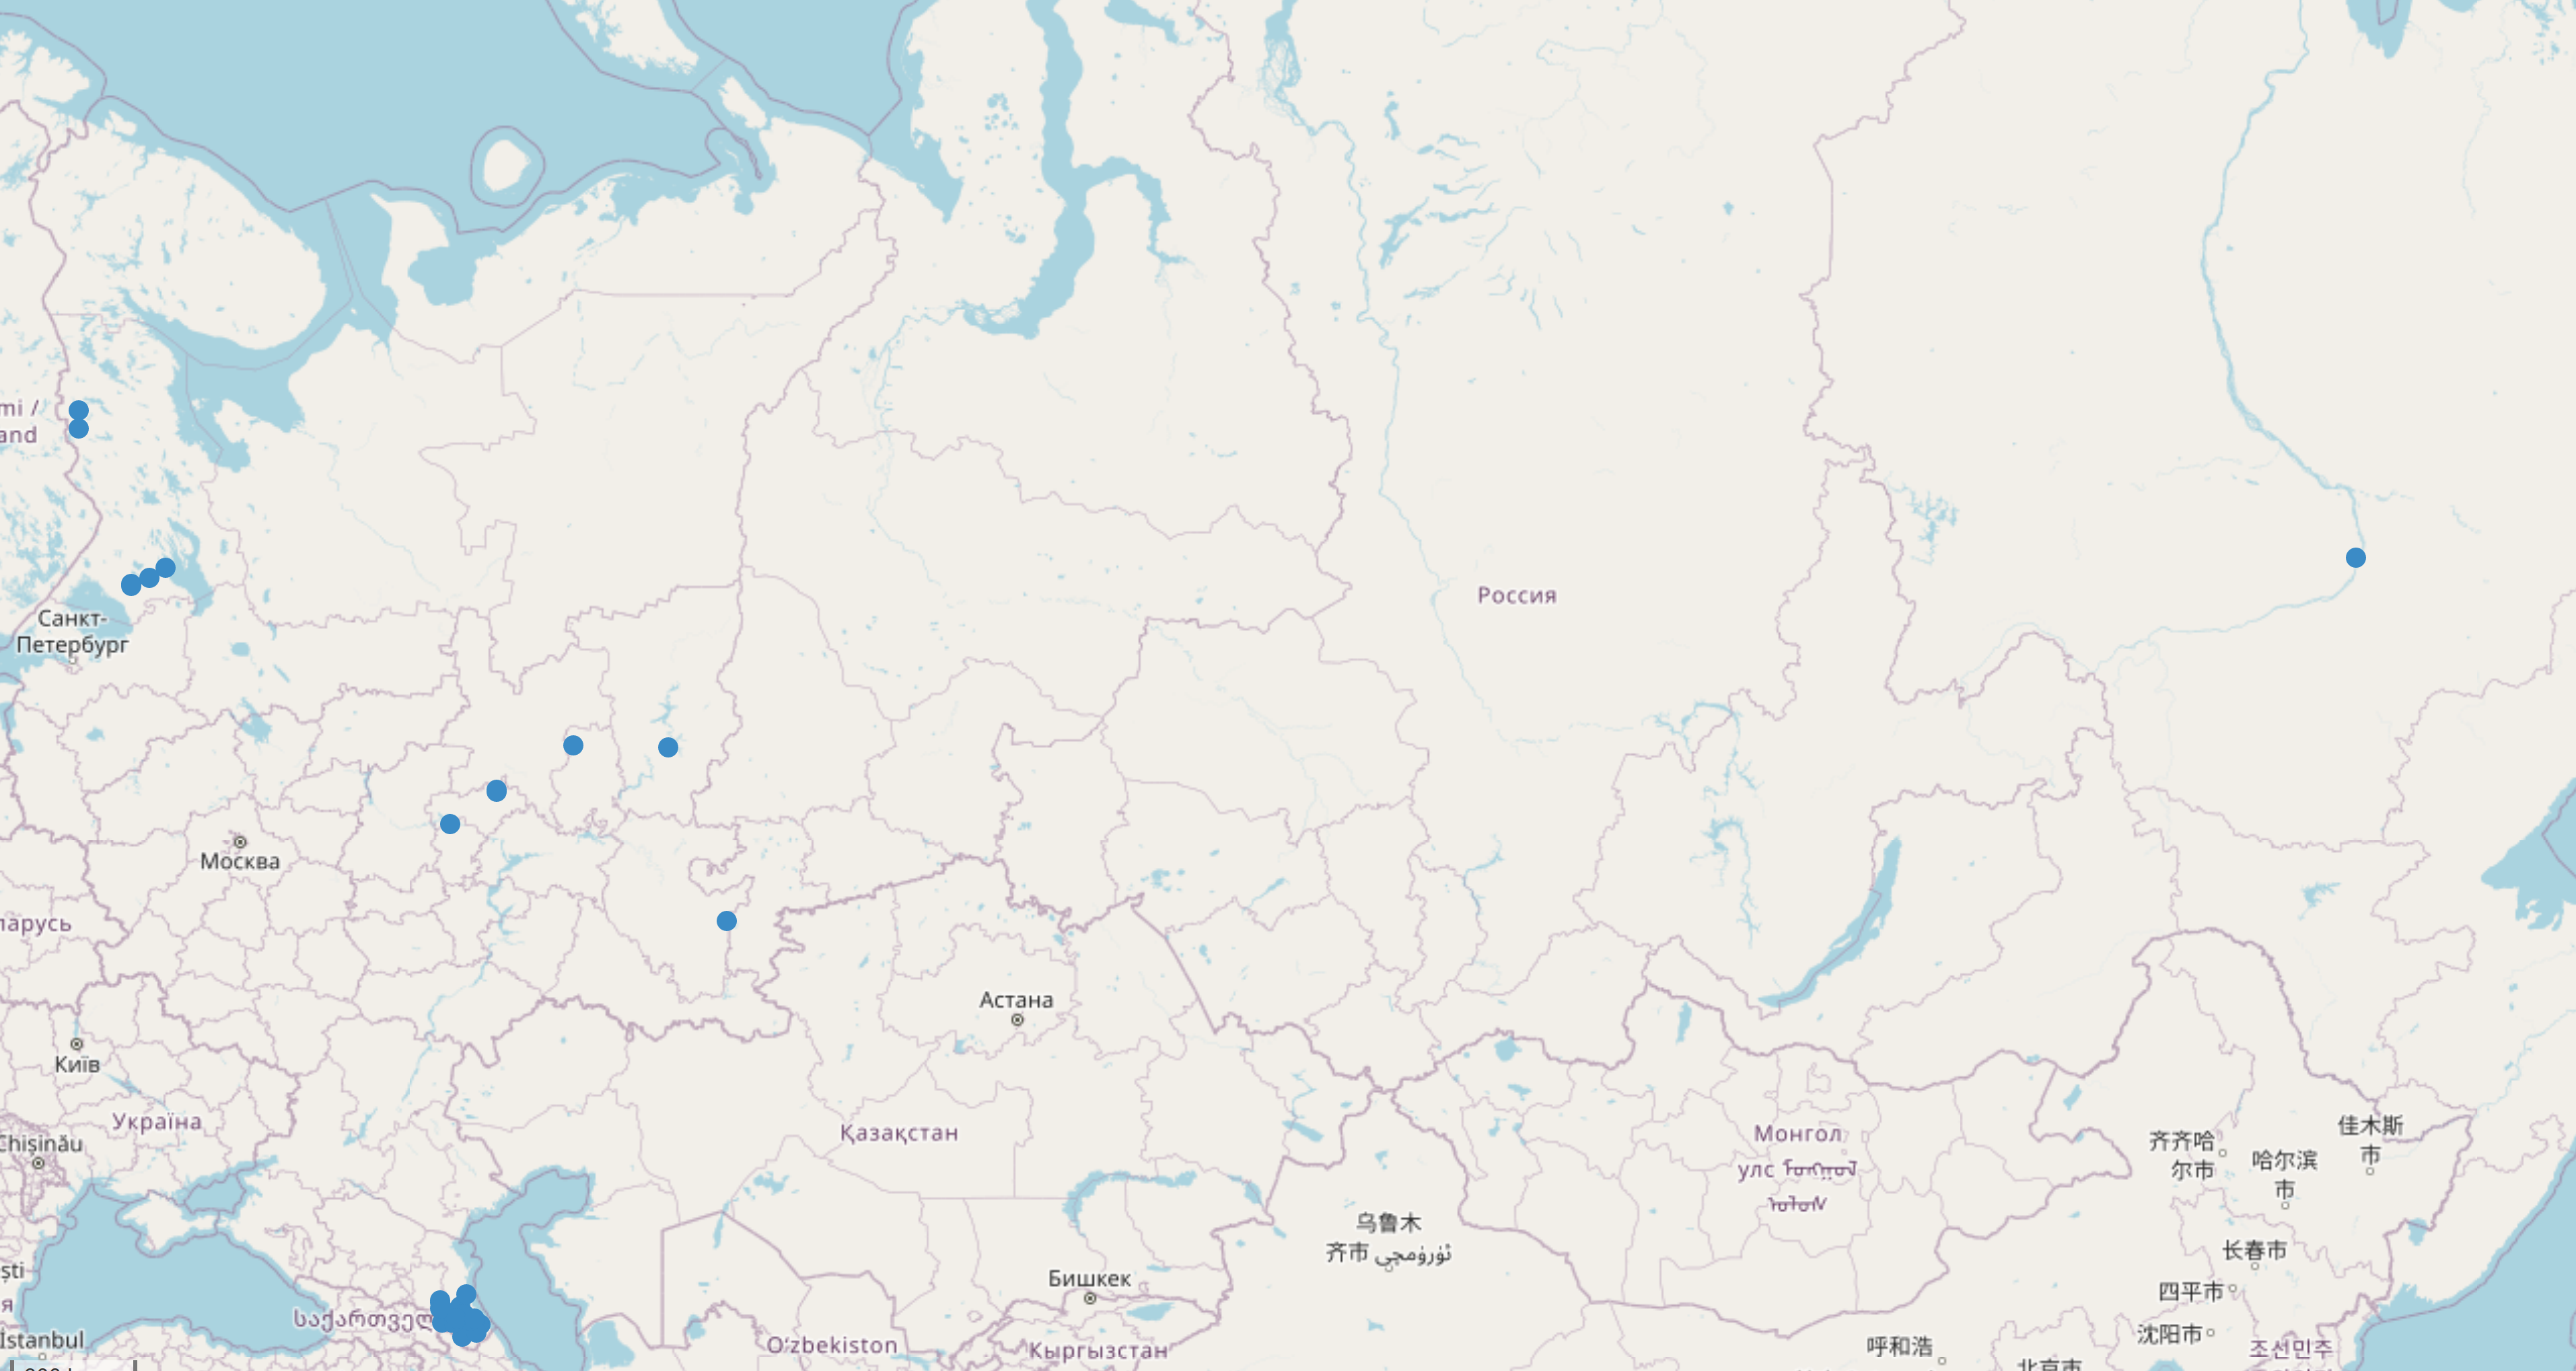
\includegraphics[width=0.99\linewidth]{images/02_bilinguals} \end{center}
\end{frame}

\begin{frame}{12 корпусов малых языков}
\protect\hypertarget{ux43aux43eux440ux43fux443ux441ux43eux432-ux43cux430ux43bux44bux445-ux44fux437ux44bux43aux43eux432}{}
\begin{center}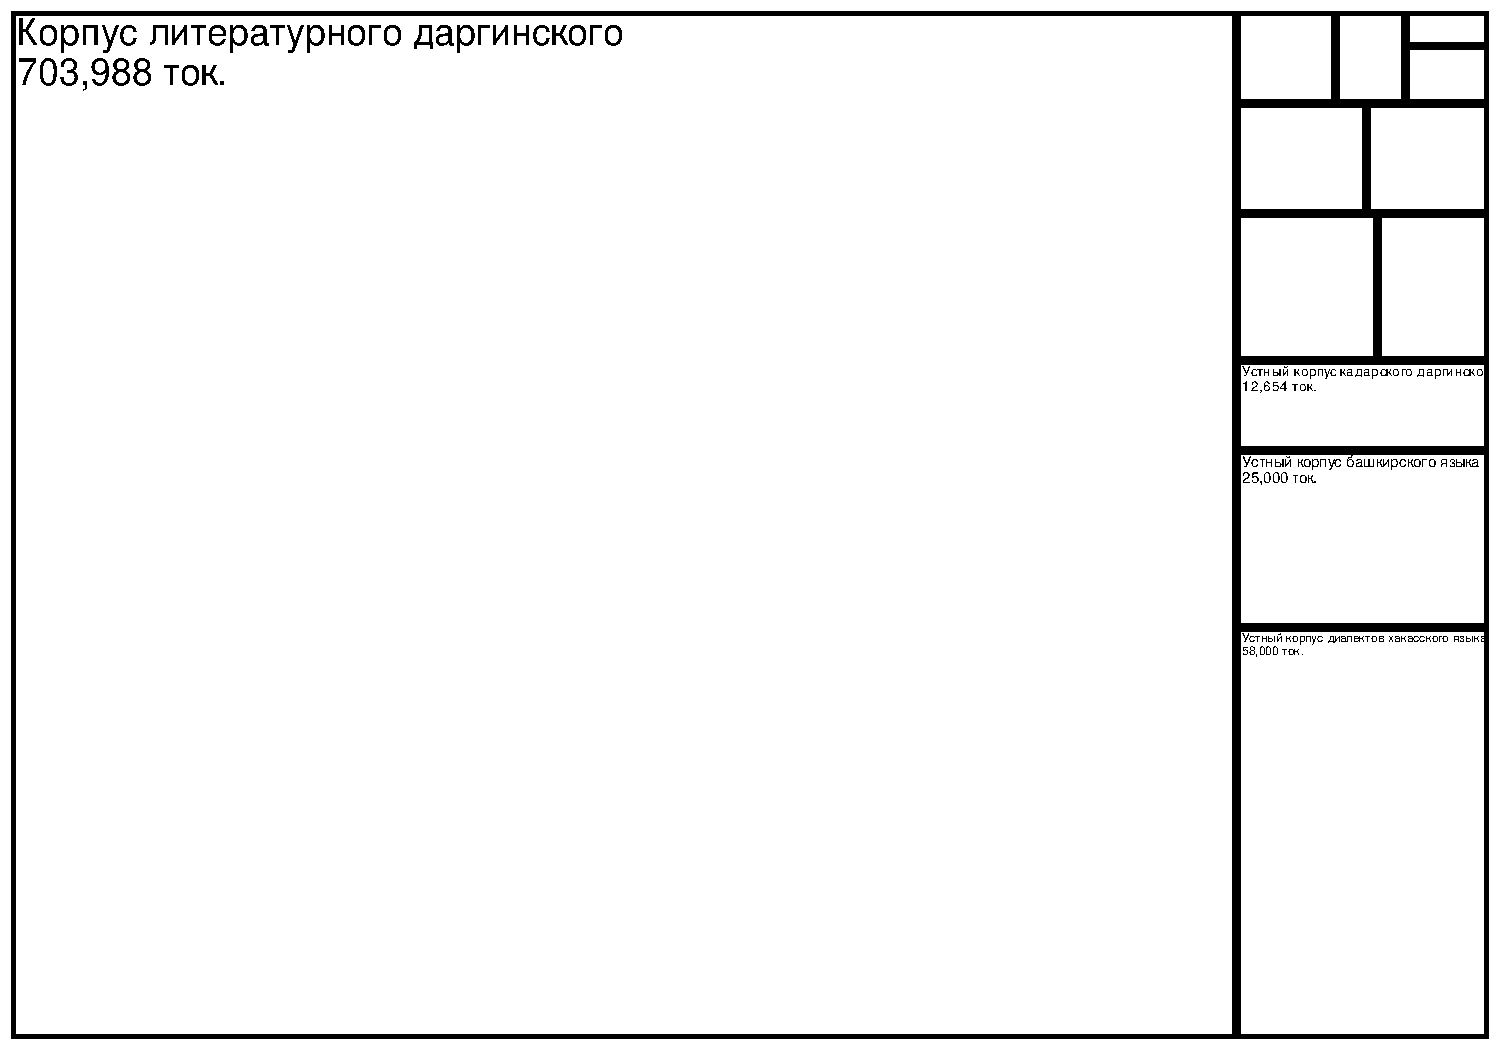
\includegraphics[width=0.99\linewidth]{2023.12.14_4nv_files/figure-beamer/unnamed-chunk-9-1} \end{center}
\end{frame}

\begin{frame}{12 корпусов малых языков}
\protect\hypertarget{ux43aux43eux440ux43fux443ux441ux43eux432-ux43cux430ux43bux44bux445-ux44fux437ux44bux43aux43eux432-1}{}
\begin{center}\includegraphics[width=0.99\linewidth]{images/03_minority} \end{center}
\end{frame}

\hypertarget{ux447ux442ux43e-ux434ux435ux43bux430ux442ux44c-ux441-ux43aux43eux440ux43fux443ux441ux430ux43cux438-ux442ux435ux43aux441ux442ux43eux432}{%
\section{Что делать с корпусами
текстов?}\label{ux447ux442ux43e-ux434ux435ux43bux430ux442ux44c-ux441-ux43aux43eux440ux43fux443ux441ux430ux43cux438-ux442ux435ux43aux441ux442ux43eux432}}

\begin{frame}{Cкорость речи \citep[382]{moroz23}}
\protect\hypertarget{cux43aux43eux440ux43eux441ux442ux44c-ux440ux435ux447ux438-moroz23-382}{}
\begin{center}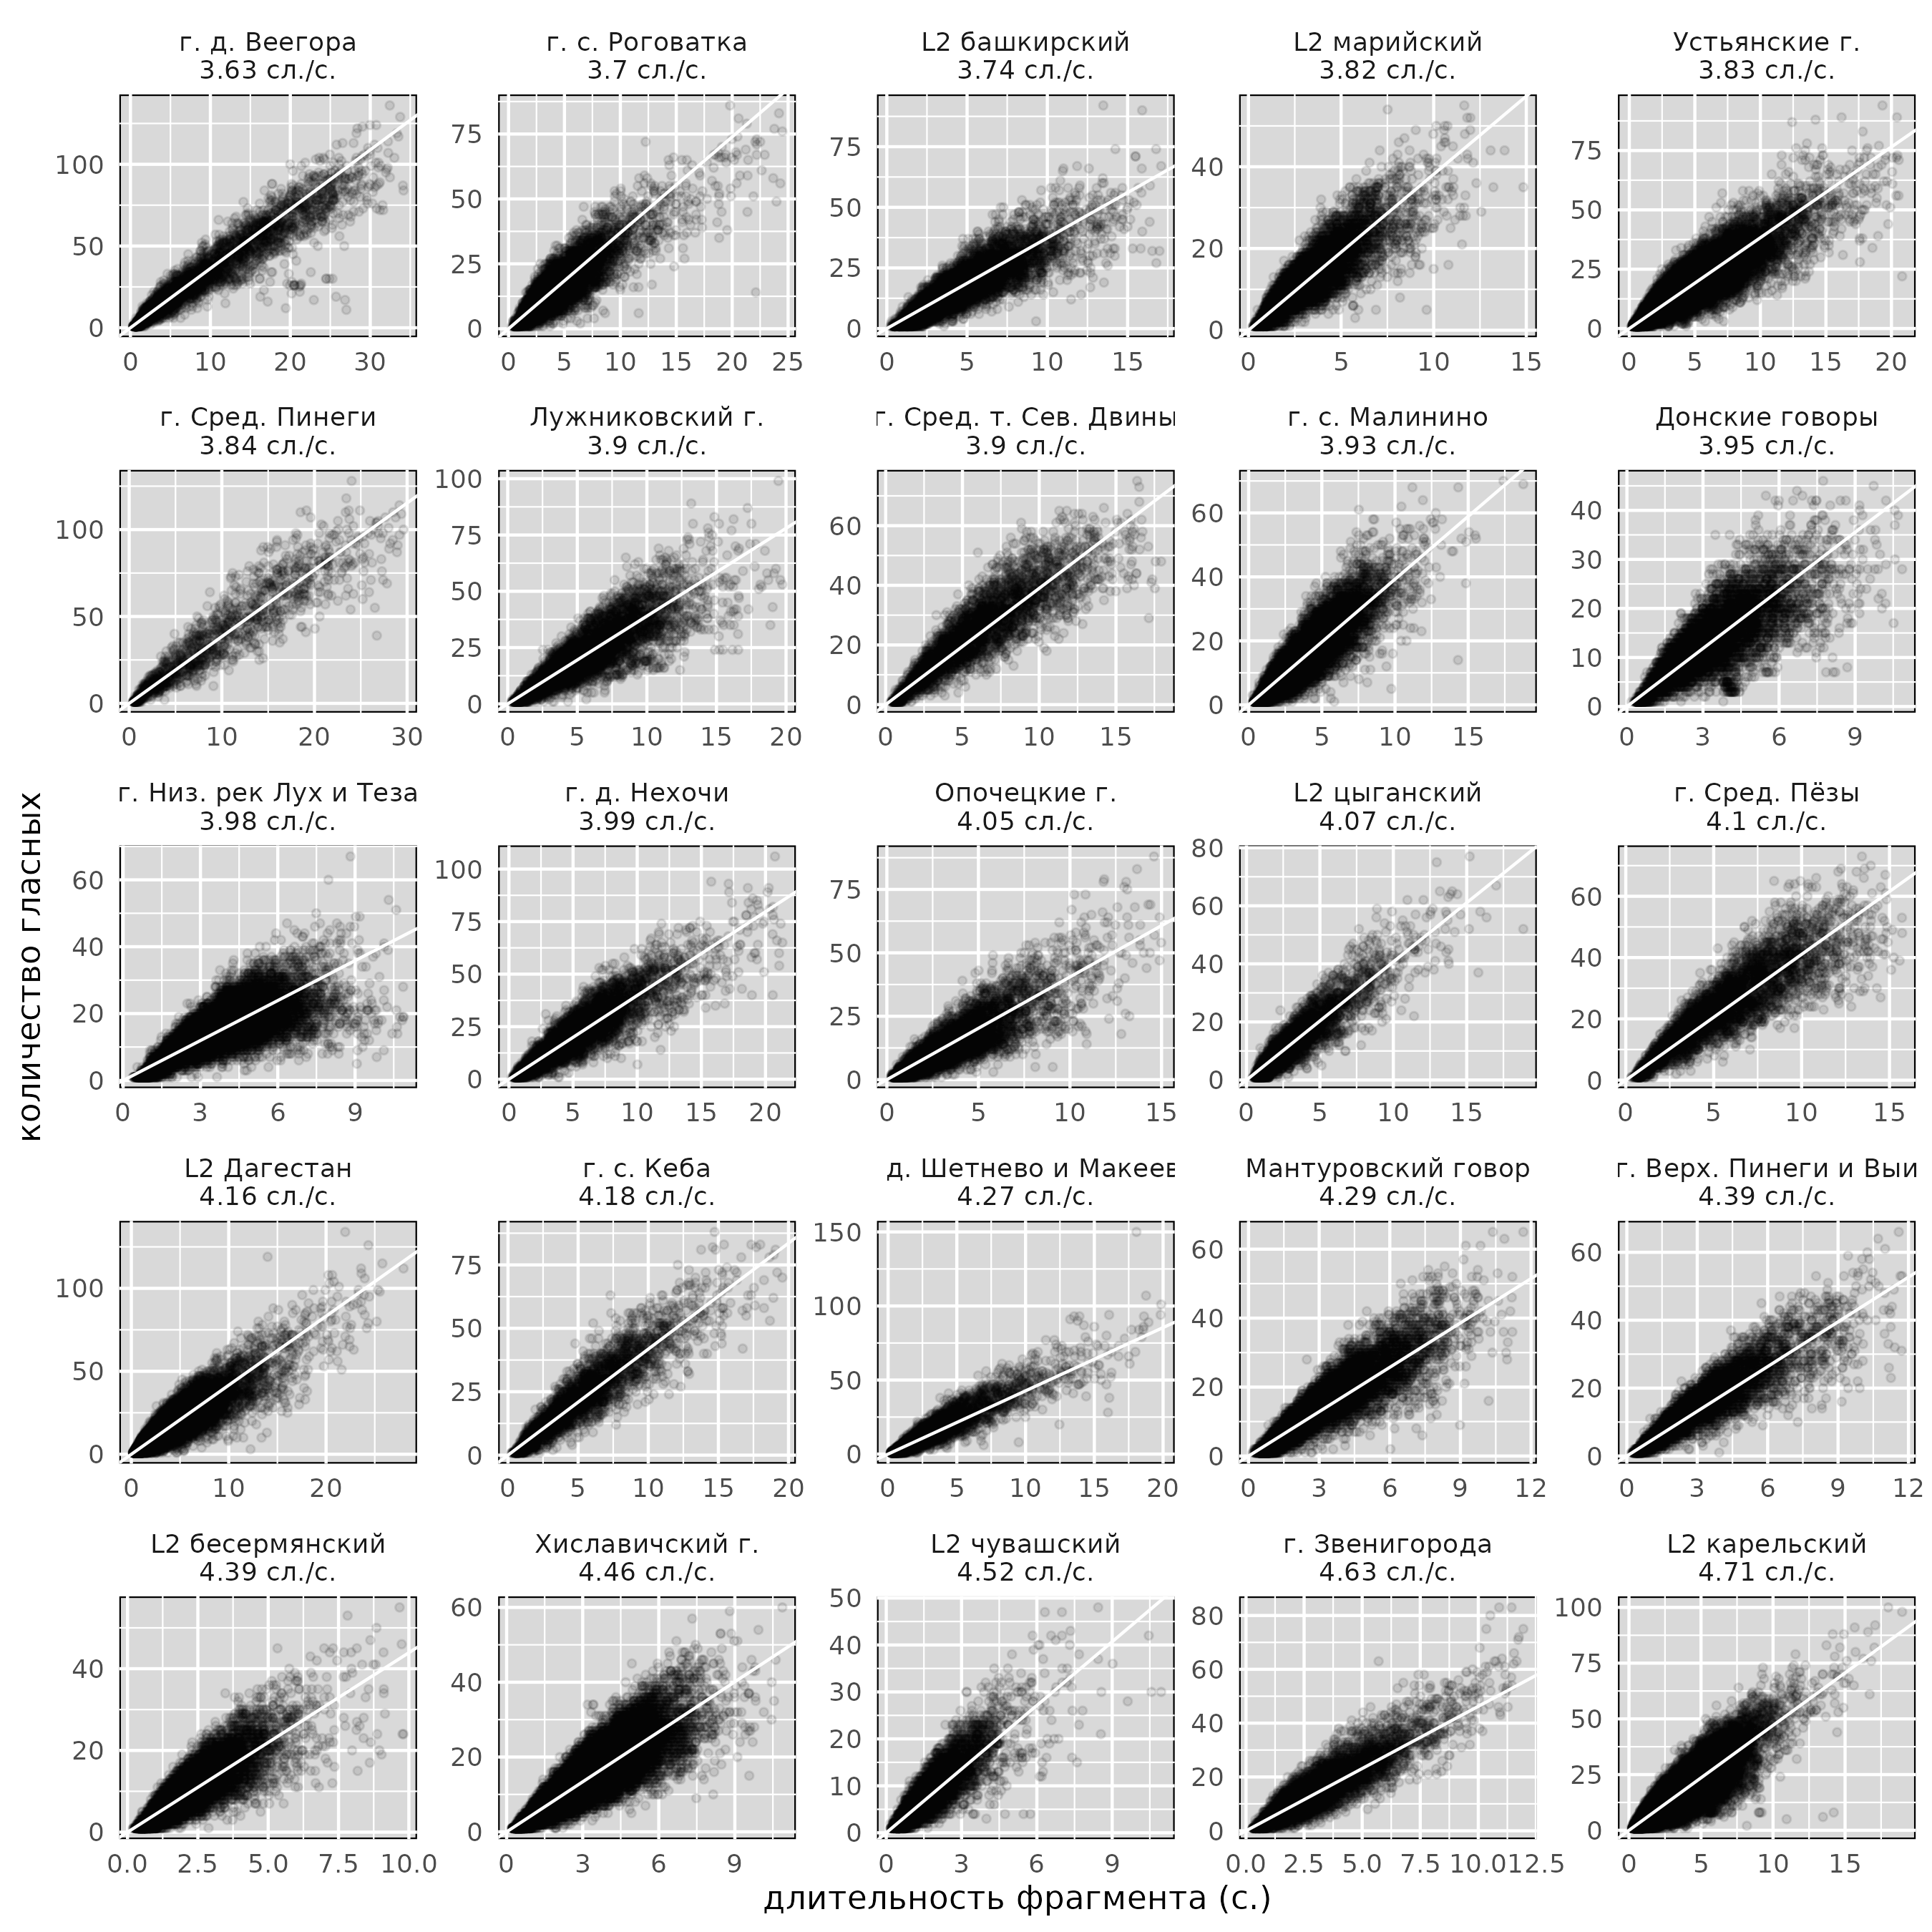
\includegraphics[width=0.8\linewidth]{images/04_speech_rate} \end{center}
\end{frame}

\begin{frame}{\href{https://lingconlab.github.io/PRuD/}{Корпус просодии
русских диалектов} \citep{knyazev24}}
\protect\hypertarget{ux43aux43eux440ux43fux443ux441-ux43fux440ux43eux441ux43eux434ux438ux438-ux440ux443ux441ux441ux43aux438ux445-ux434ux438ux430ux43bux435ux43aux442ux43eux432-knyazev24}{}
\begin{center}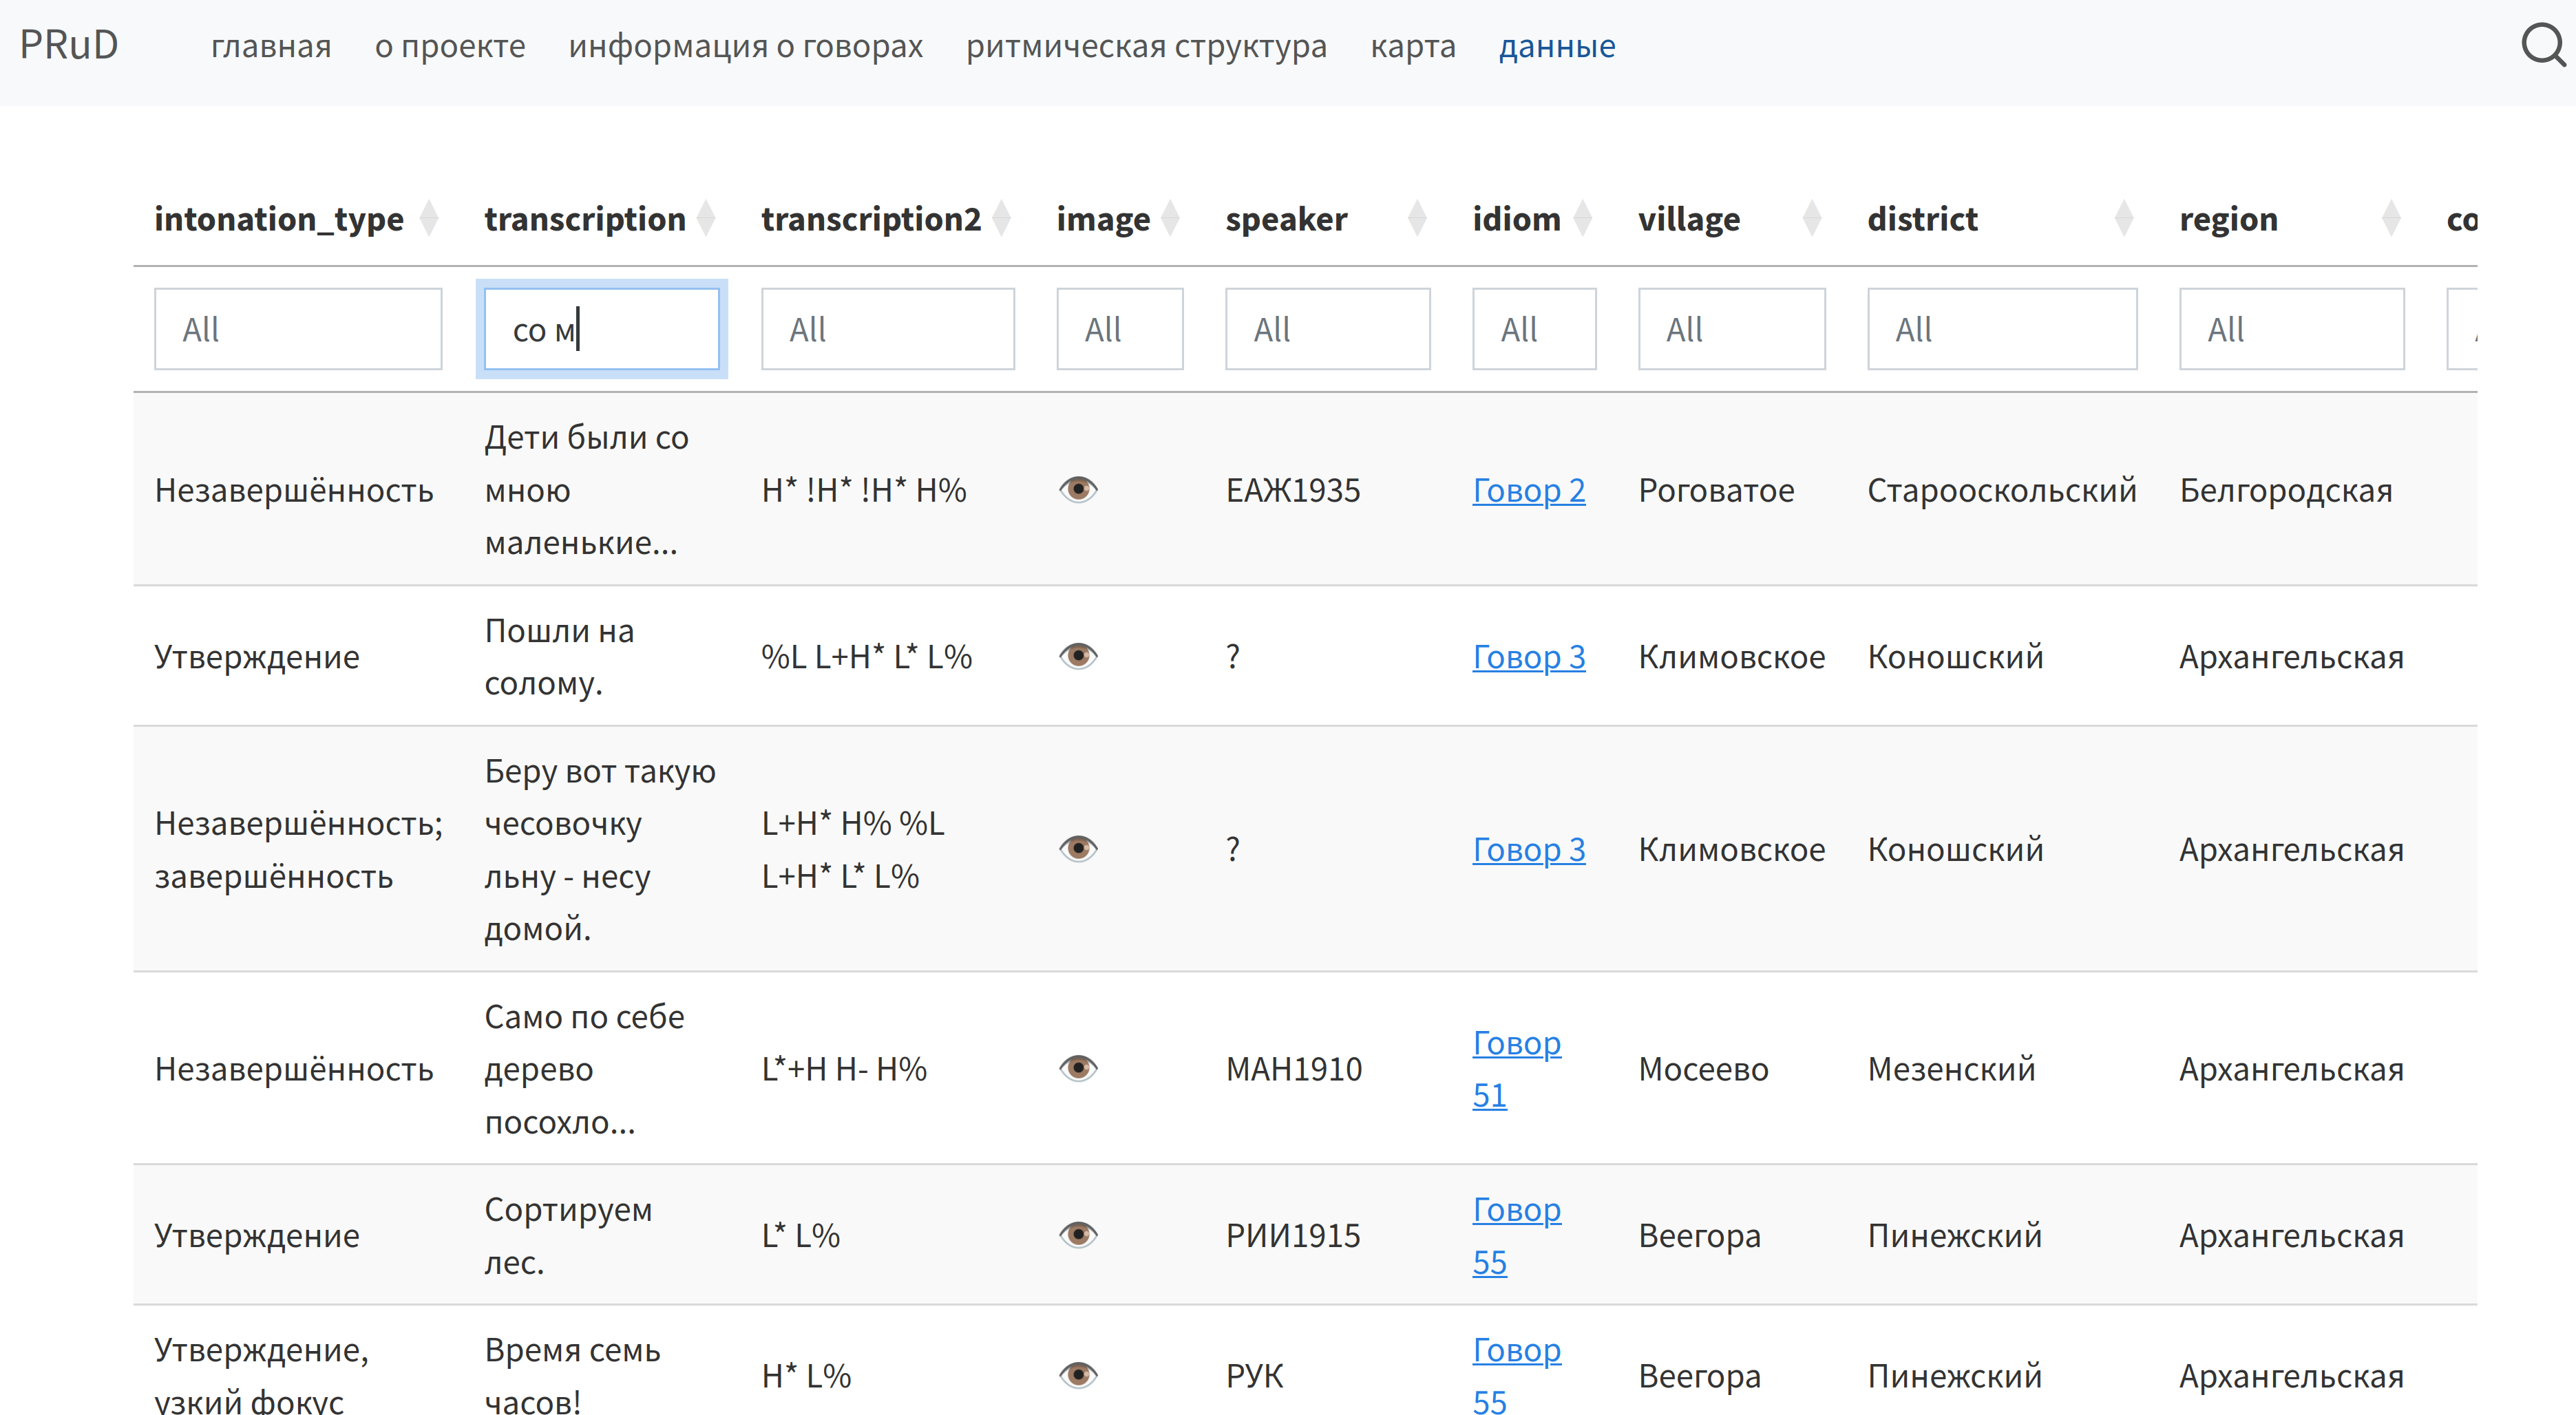
\includegraphics[width=0.99\linewidth]{images/05_PRuD} \end{center}
\end{frame}

\begin{frame}{Исследование вариативности}
\protect\hypertarget{ux438ux441ux441ux43bux435ux434ux43eux432ux430ux43dux438ux435-ux432ux430ux440ux438ux430ux442ux438ux432ux43dux43eux441ux442ux438}{}
\begin{figure}

{\centering 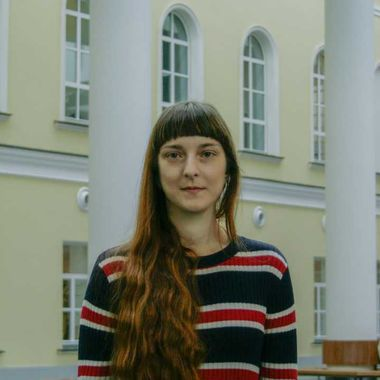
\includegraphics[width=0.24\linewidth]{images/sveta} 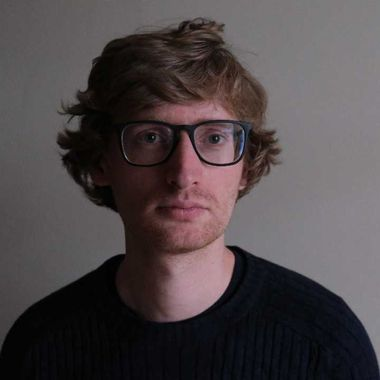
\includegraphics[width=0.24\linewidth]{images/garik} 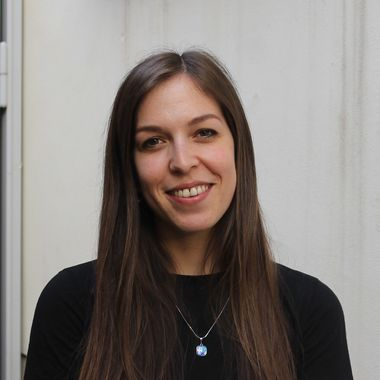
\includegraphics[width=0.24\linewidth]{images/chiara} 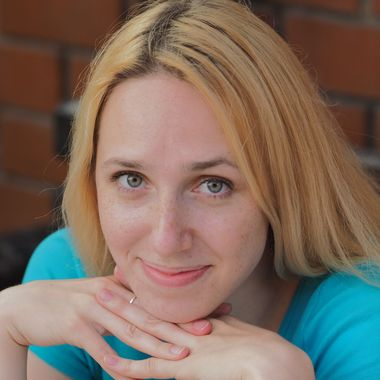
\includegraphics[width=0.24\linewidth]{images/nastya} 

}

\caption{С. С. Земичева, Г. А. Мороз, К. Наккарато, А. В. Яковлева}\label{fig:unnamed-chunk-14}
\end{figure}

Грант РНФ (24-28-01097) ``Исследование вариативности билингвального и
диалектного русского языка на материале устных корпусов''
\end{frame}

\hypertarget{ux43eux43fux44bux442-ux437ux435ux440ux43aux430ux43bux44cux43dux43eux439-ux43bux430ux431ux43eux440ux430ux442ux43eux440ux438ux438-ux441-ux44eux436ux43dux44bux43c-ux444ux435ux434ux435ux440ux430ux43bux44cux43dux44bux43c-ux443ux43dux438ux432ux435ux440ux441ux438ux442ux435ux442ux43eux43c}{%
\section{Опыт зеркальной лаборатории с Южным Федеральным
Университетом}\label{ux43eux43fux44bux442-ux437ux435ux440ux43aux430ux43bux44cux43dux43eux439-ux43bux430ux431ux43eux440ux430ux442ux43eux440ux438ux438-ux441-ux44eux436ux43dux44bux43c-ux444ux435ux434ux435ux440ux430ux43bux44cux43dux44bux43c-ux443ux43dux438ux432ux435ux440ux441ux438ux442ux435ux442ux43eux43c}}

\begin{frame}{Зеркальная лаборатория с ЮФУ}
\protect\hypertarget{ux437ux435ux440ux43aux430ux43bux44cux43dux430ux44f-ux43bux430ux431ux43eux440ux430ux442ux43eux440ux438ux44f-ux441-ux44eux444ux443}{}
\begin{itemize}
\tightlist
\item
  проходила 2020-2023 под руководством Елены Михайловны Севериной
\end{itemize}

\begin{center}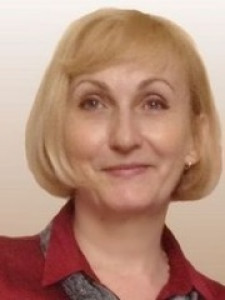
\includegraphics[width=0.3\linewidth]{images/severina} \end{center}
\end{frame}

\begin{frame}{Зеркальная лаборатория с ЮФУ}
\protect\hypertarget{ux437ux435ux440ux43aux430ux43bux44cux43dux430ux44f-ux43bux430ux431ux43eux440ux430ux442ux43eux440ux438ux44f-ux441-ux44eux444ux443-1}{}
В рамках зеркальной лаборатории велась работа по трем направлениям:

\begin{itemize}
\tightlist
\item
  \textbf{Проект Digital Chekhov}: создание многоуровневой
  (семантической) разметки собрания произведений А. П. Чехова
\item
  \textbf{Устный корпус донских диалектов}: аннотация аудиозаписей и
  создание интерфейса устного корпуса
\item
  \textbf{Русский учебный корпус}: образцы устной и письменной речи
  нестандартных говорящих на русском языке, изучающих русский язык как
  иностранный
\end{itemize}
\end{frame}

\begin{frame}{Digital Chekhov}
\protect\hypertarget{digital-chekhov}{}
\begin{itemize}
\tightlist
\item
  \url{https://chekhov-digital.sfedu.ru/}
\end{itemize}

\begin{center}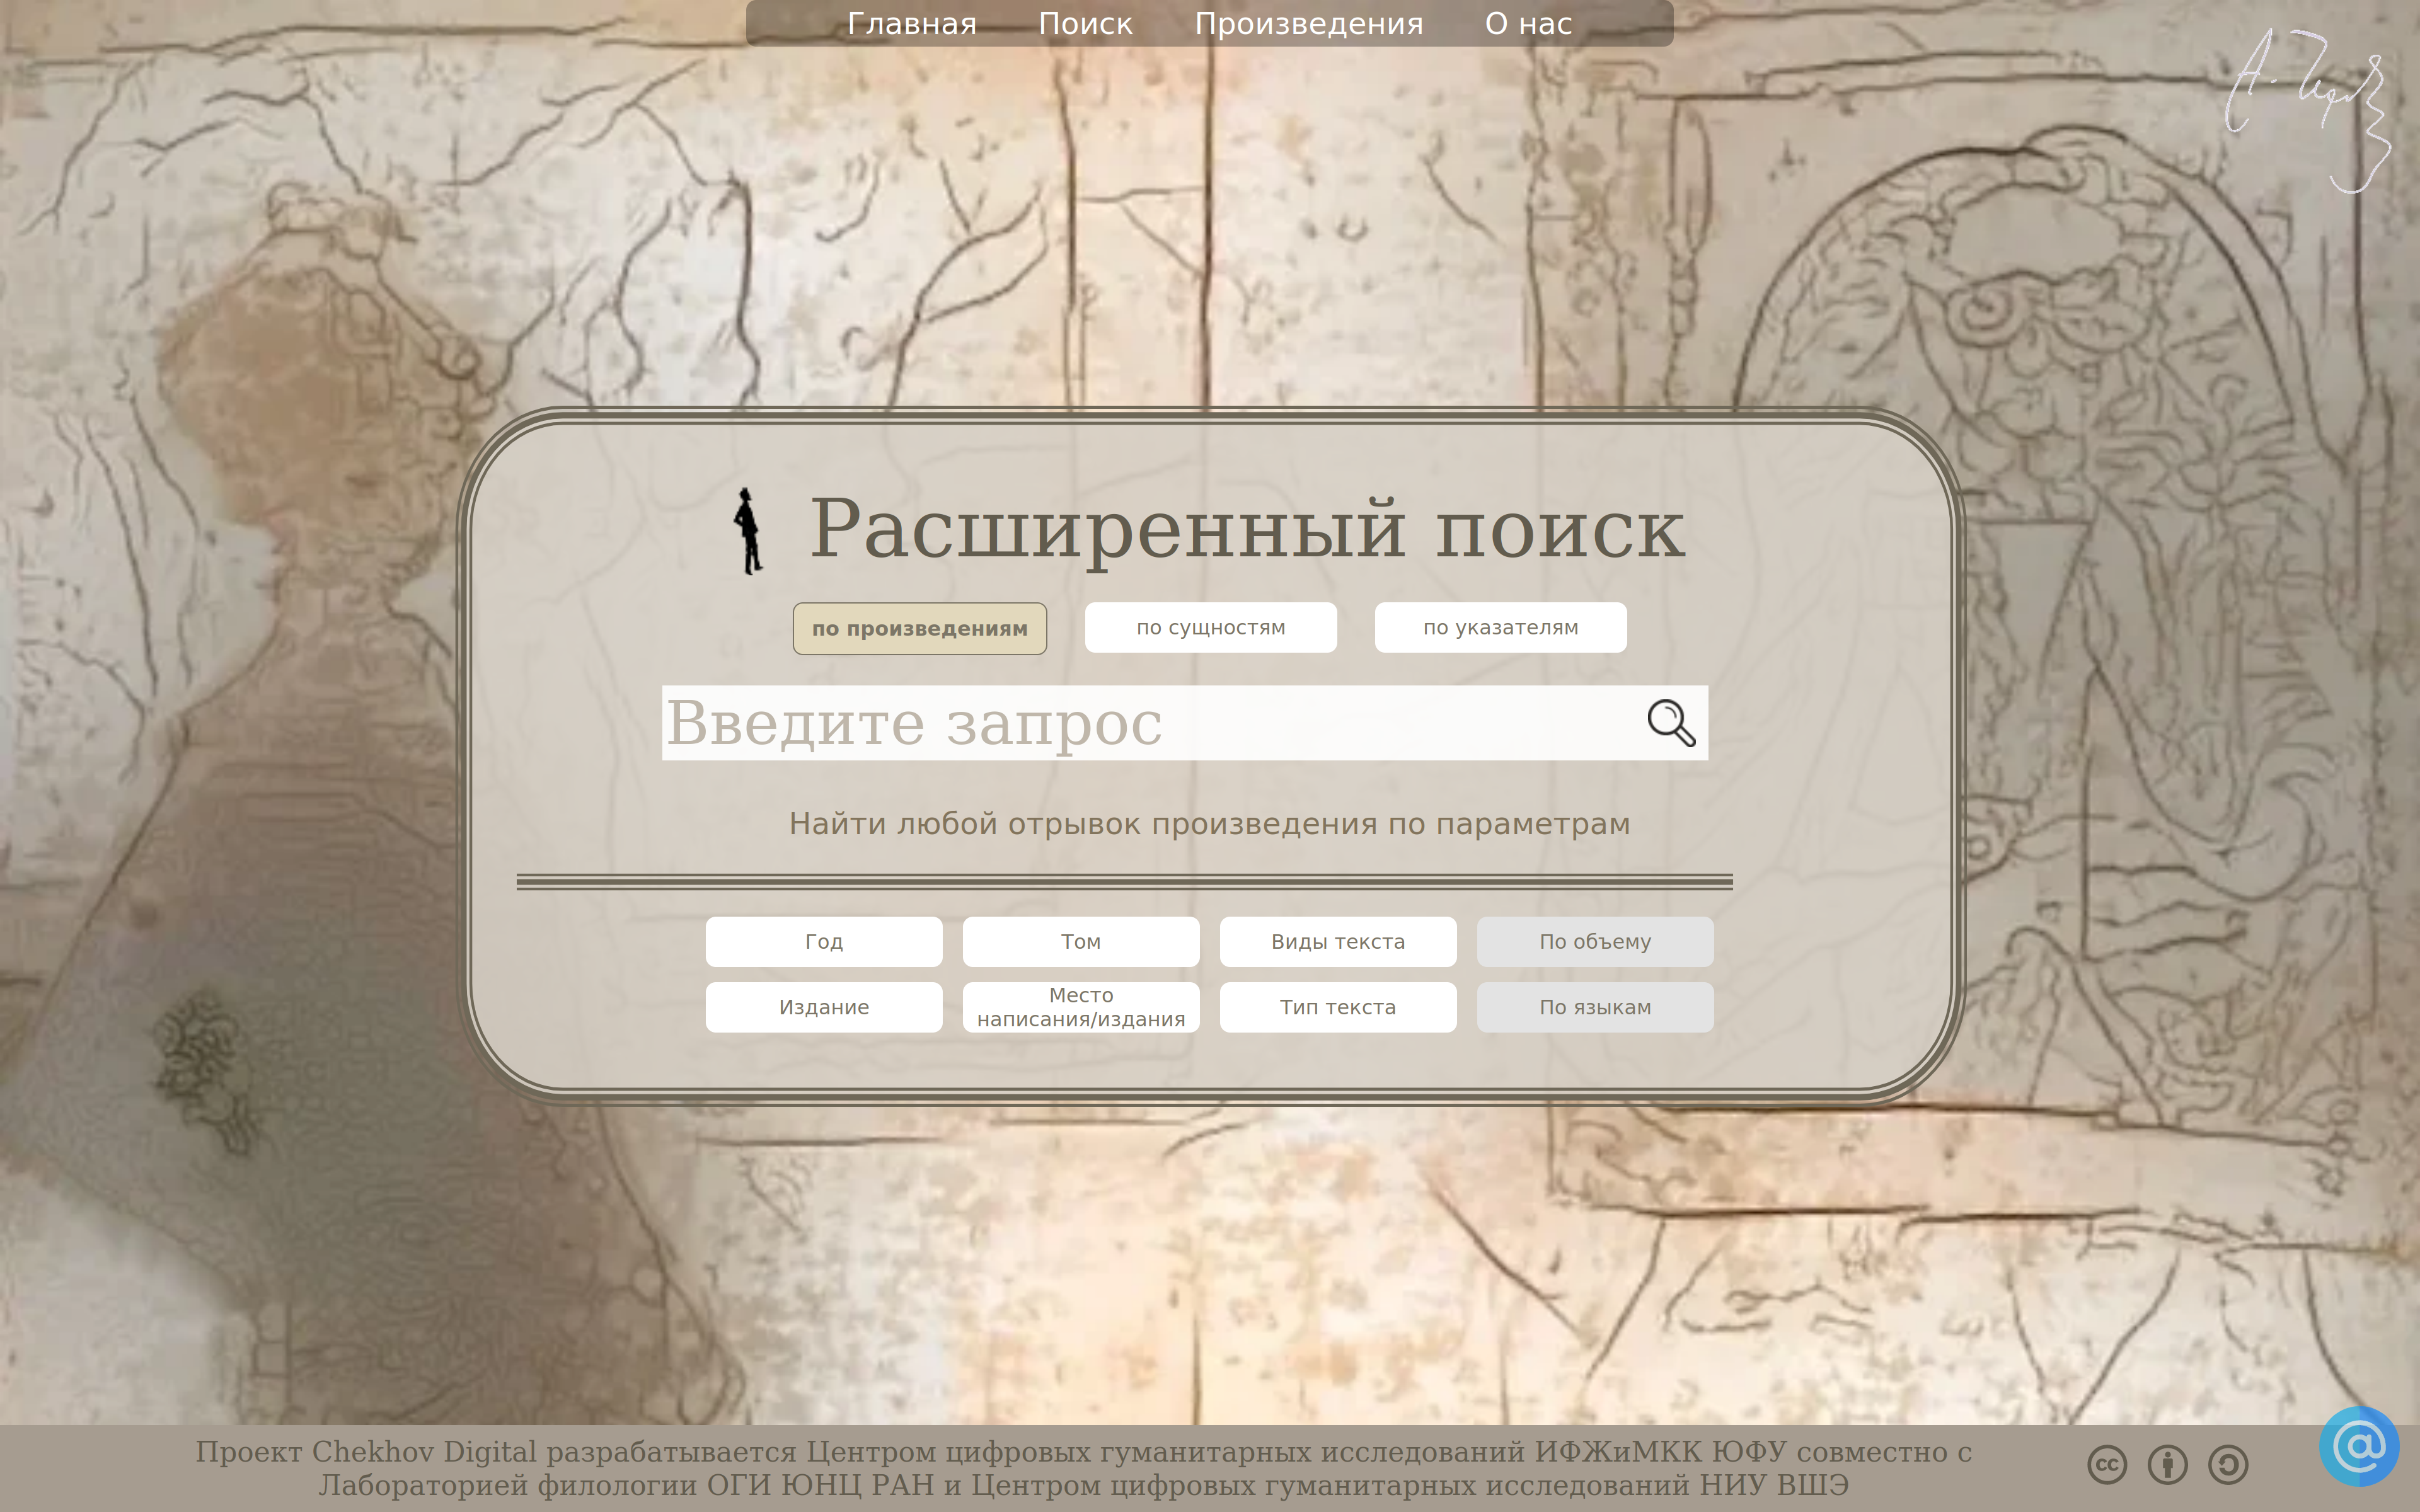
\includegraphics[width=0.95\linewidth]{images/06_digital_chekhov} \end{center}
\end{frame}

\begin{frame}{Устный корпус донских диалектов}
\protect\hypertarget{ux443ux441ux442ux43dux44bux439-ux43aux43eux440ux43fux443ux441-ux434ux43eux43dux441ux43aux438ux445-ux434ux438ux430ux43bux435ux43aux442ux43eux432}{}
\begin{itemize}
\tightlist
\item
  \url{http://lingconlab.ru/don_rnd}
\end{itemize}

\begin{center}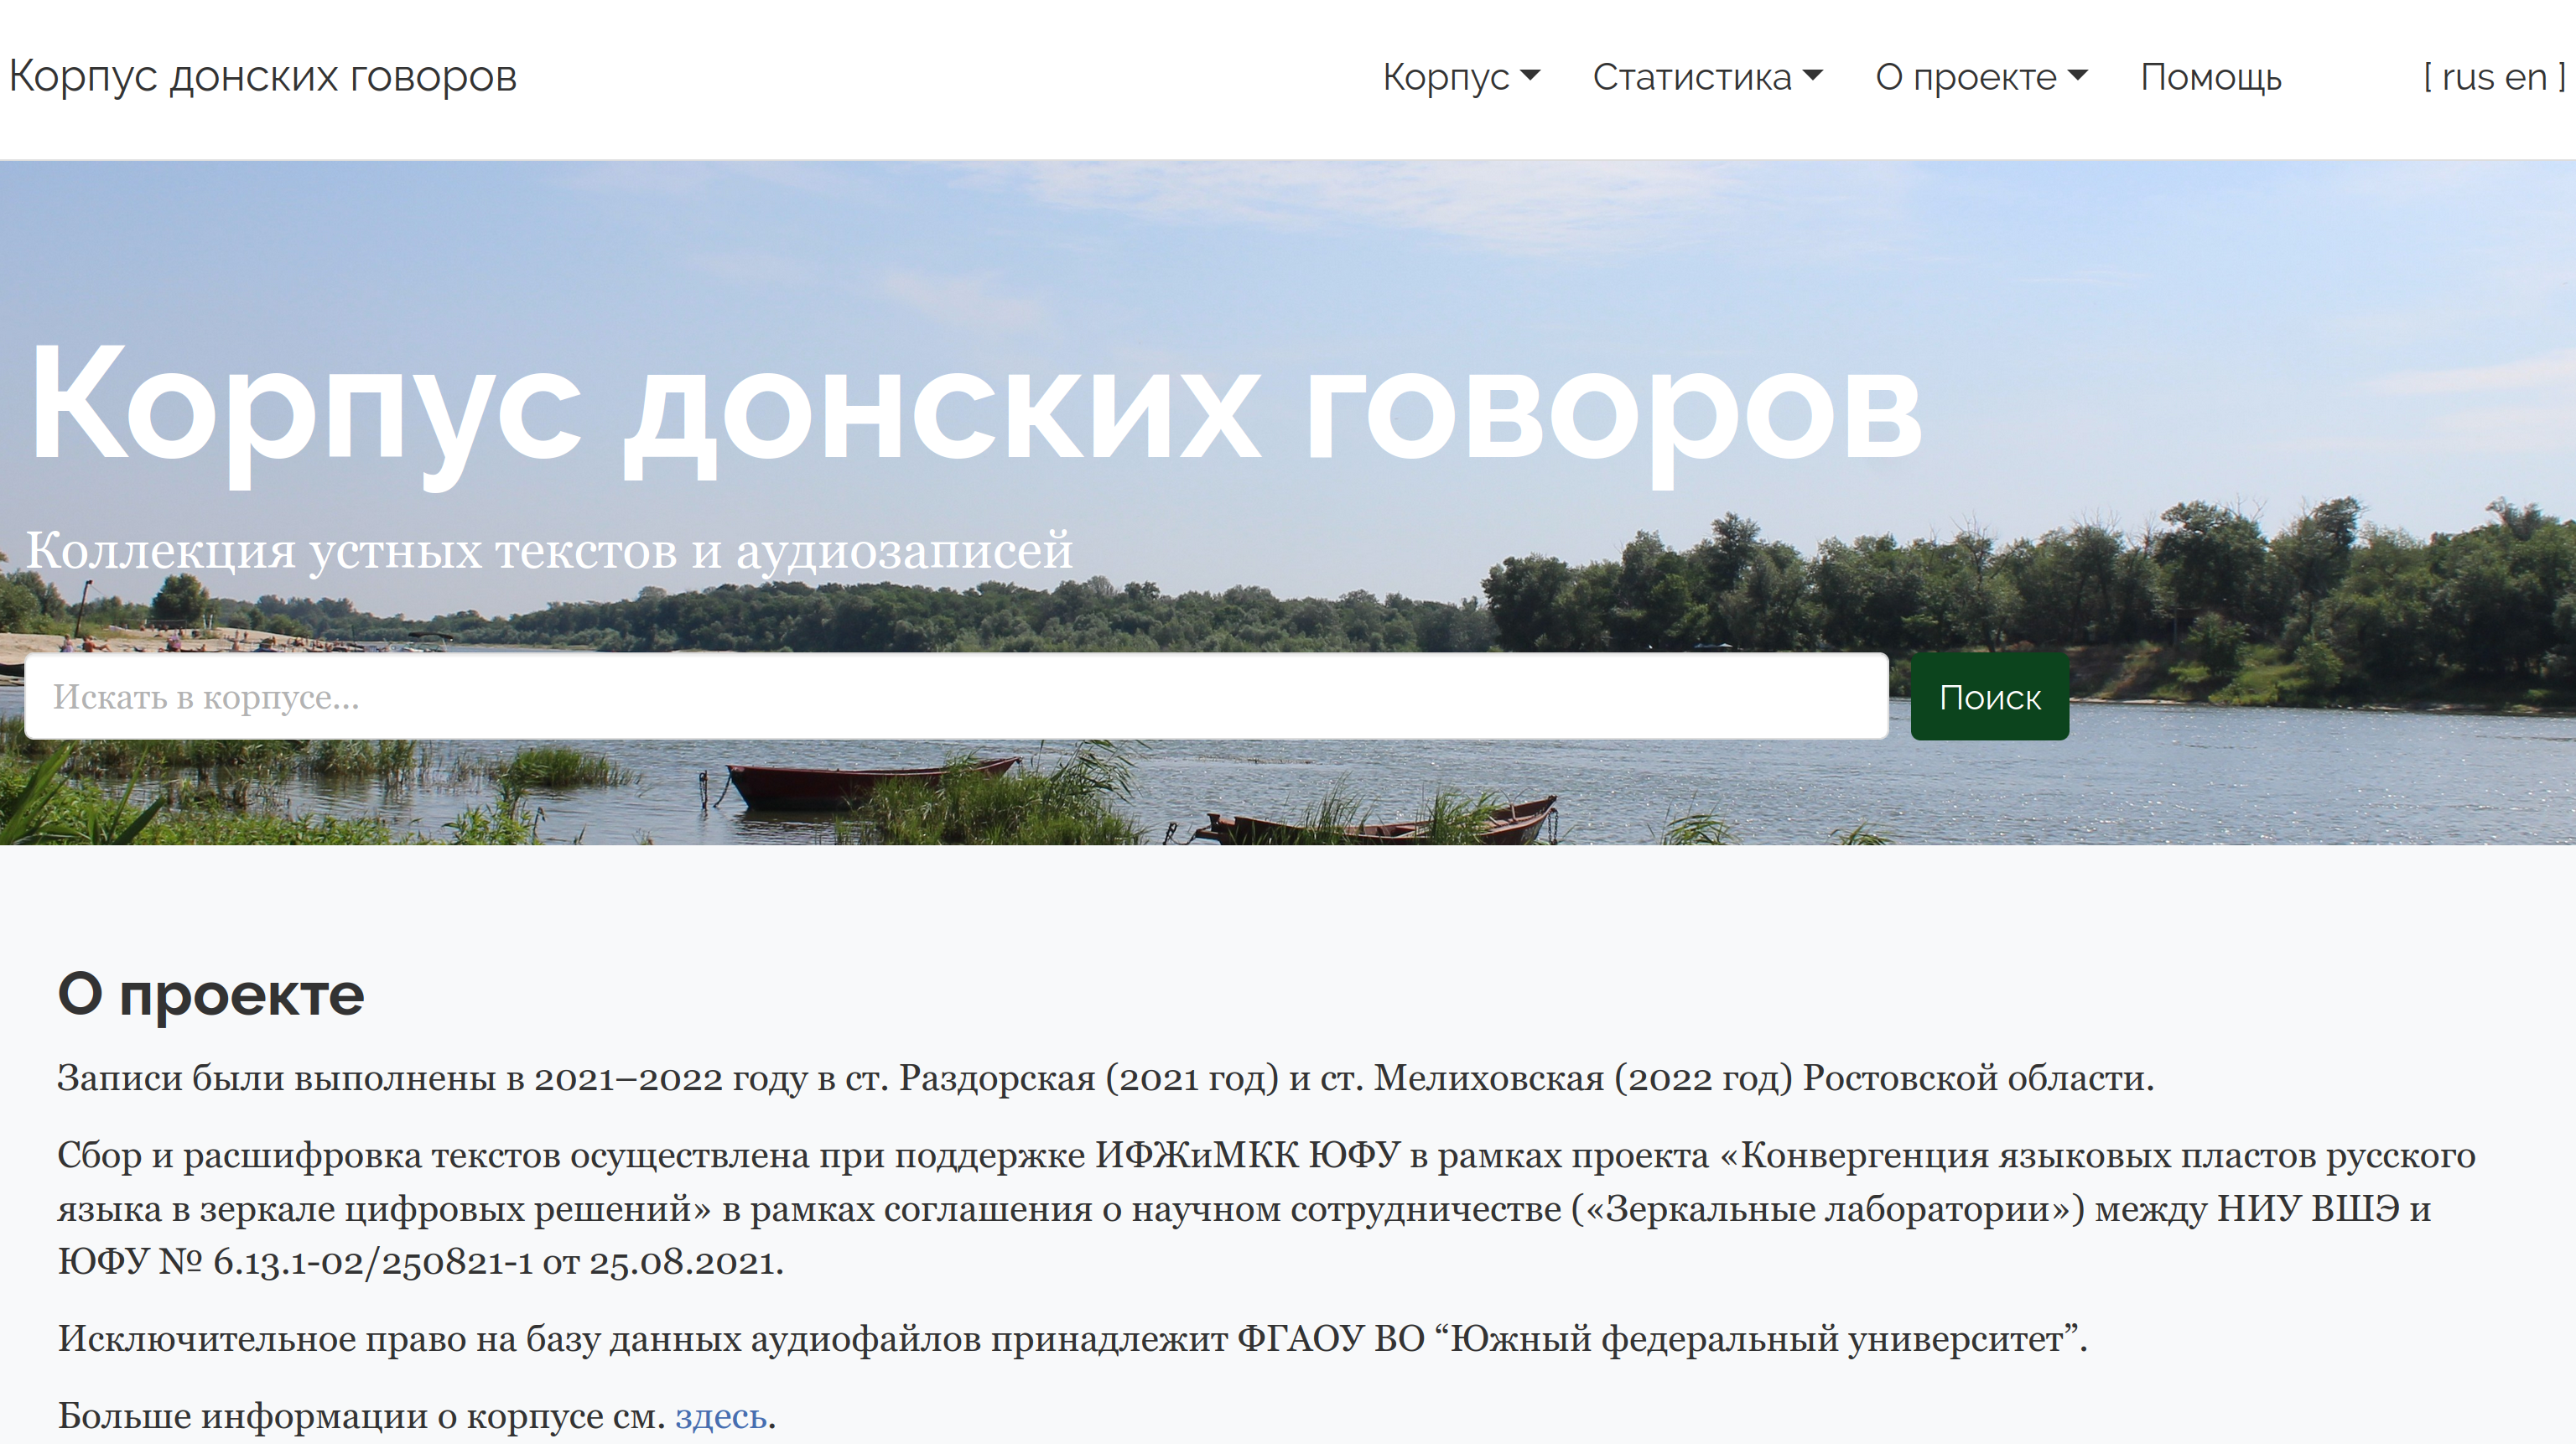
\includegraphics[width=0.98\linewidth]{images/don1} \end{center}
\end{frame}

\begin{frame}{Устный корпус донских диалектов}
\protect\hypertarget{ux443ux441ux442ux43dux44bux439-ux43aux43eux440ux43fux443ux441-ux434ux43eux43dux441ux43aux438ux445-ux434ux438ux430ux43bux435ux43aux442ux43eux432-1}{}
\begin{itemize}
\tightlist
\item
  \url{http://lingconlab.ru/don_rnd}
\end{itemize}

\begin{center}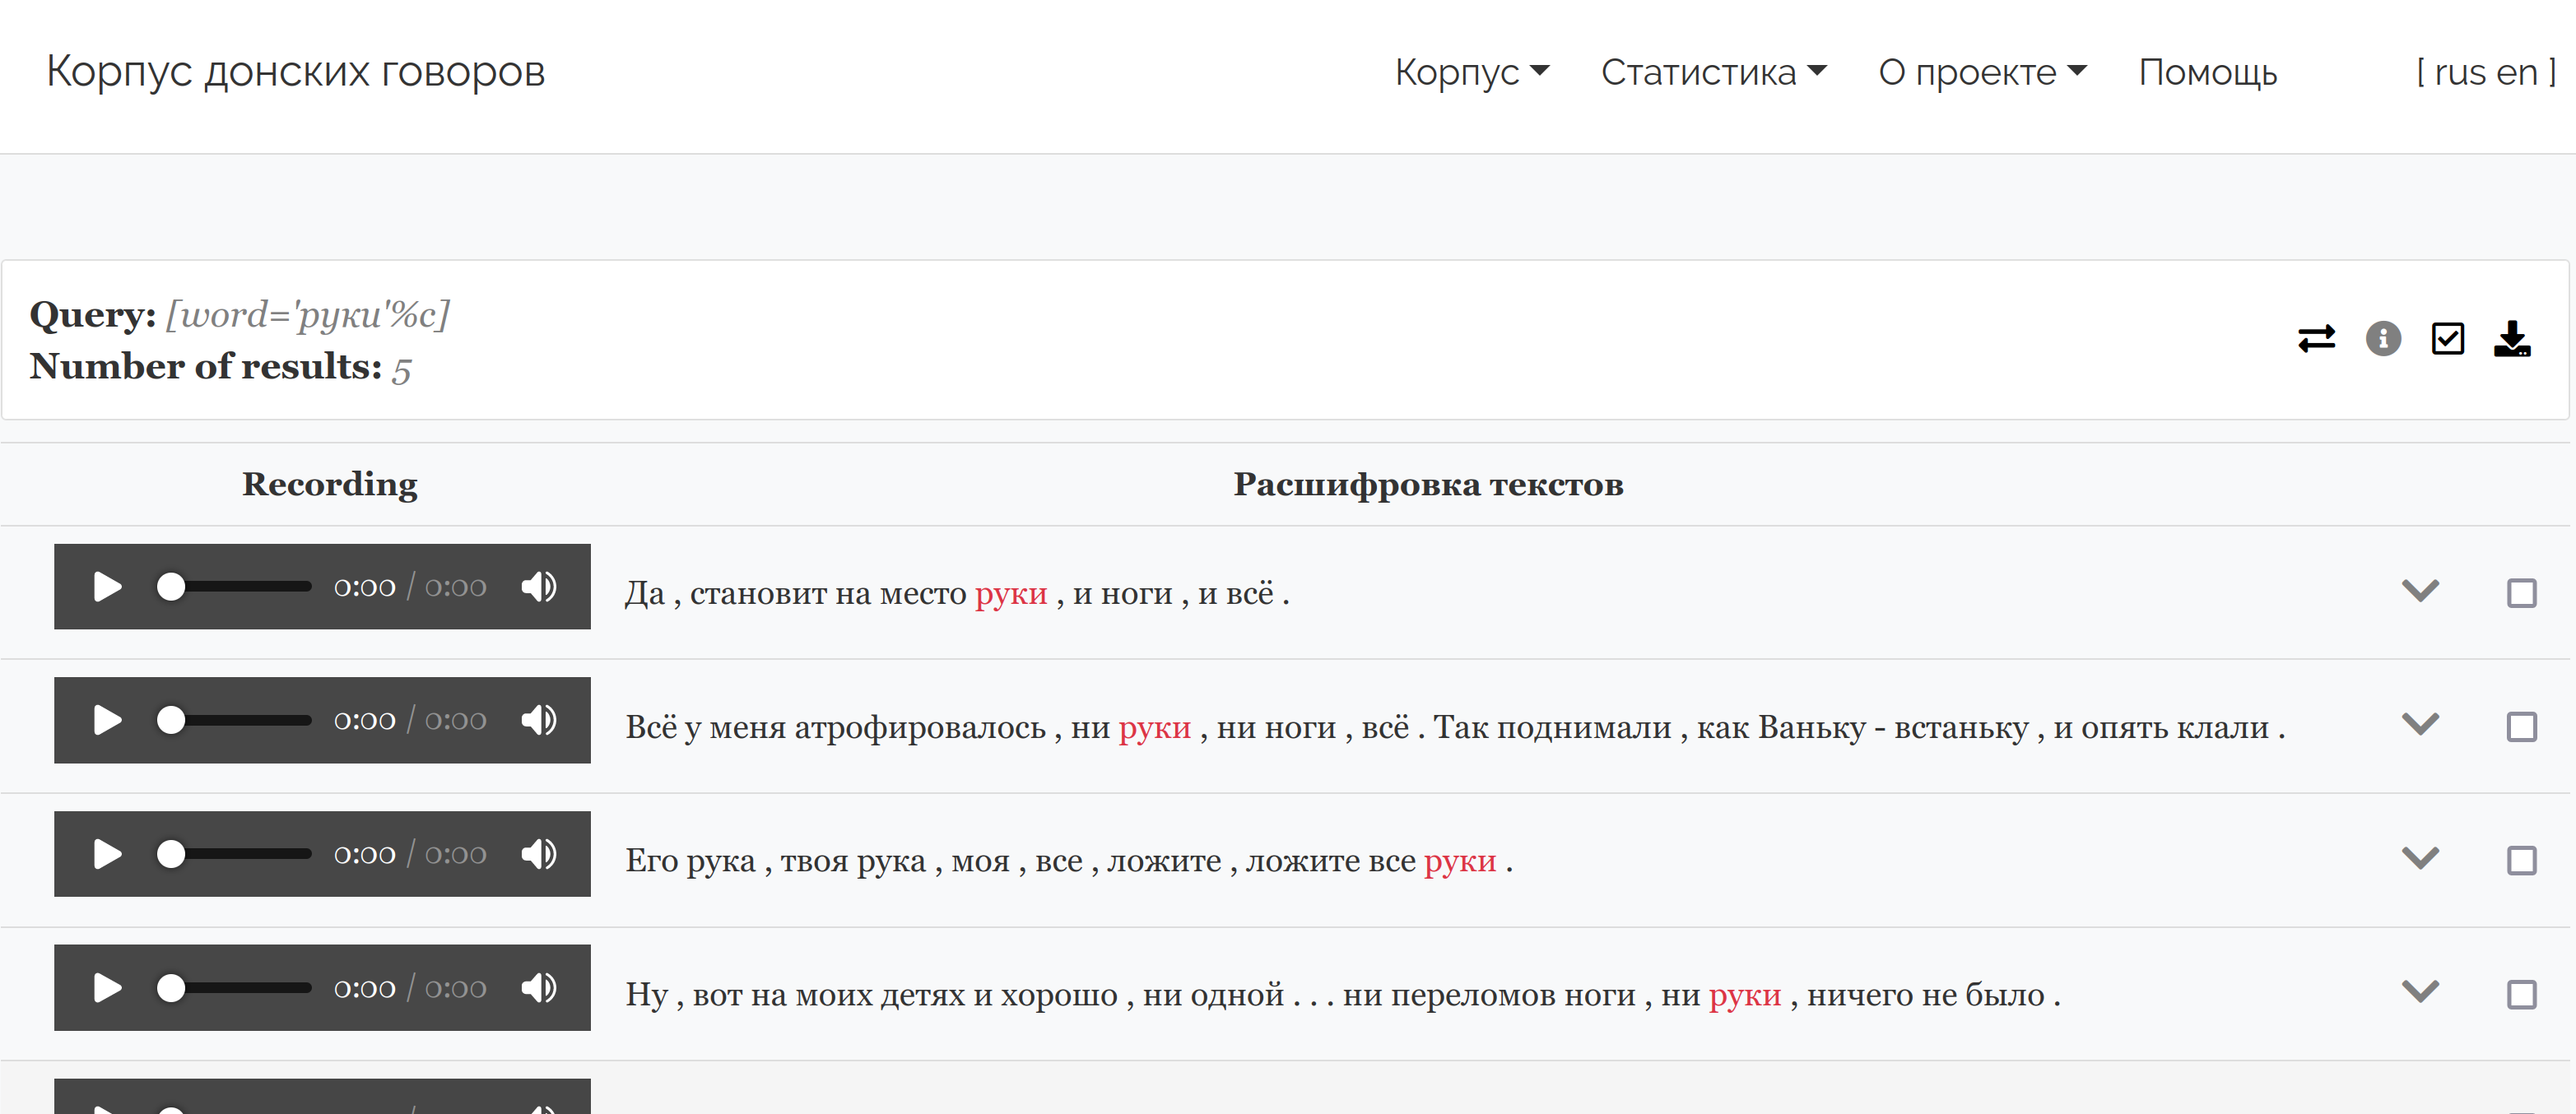
\includegraphics[width=0.98\linewidth]{images/don2} \end{center}
\end{frame}

\begin{frame}{Русский учебный корпус}
\protect\hypertarget{ux440ux443ux441ux441ux43aux438ux439-ux443ux447ux435ux431ux43dux44bux439-ux43aux43eux440ux43fux443ux441}{}
\begin{center}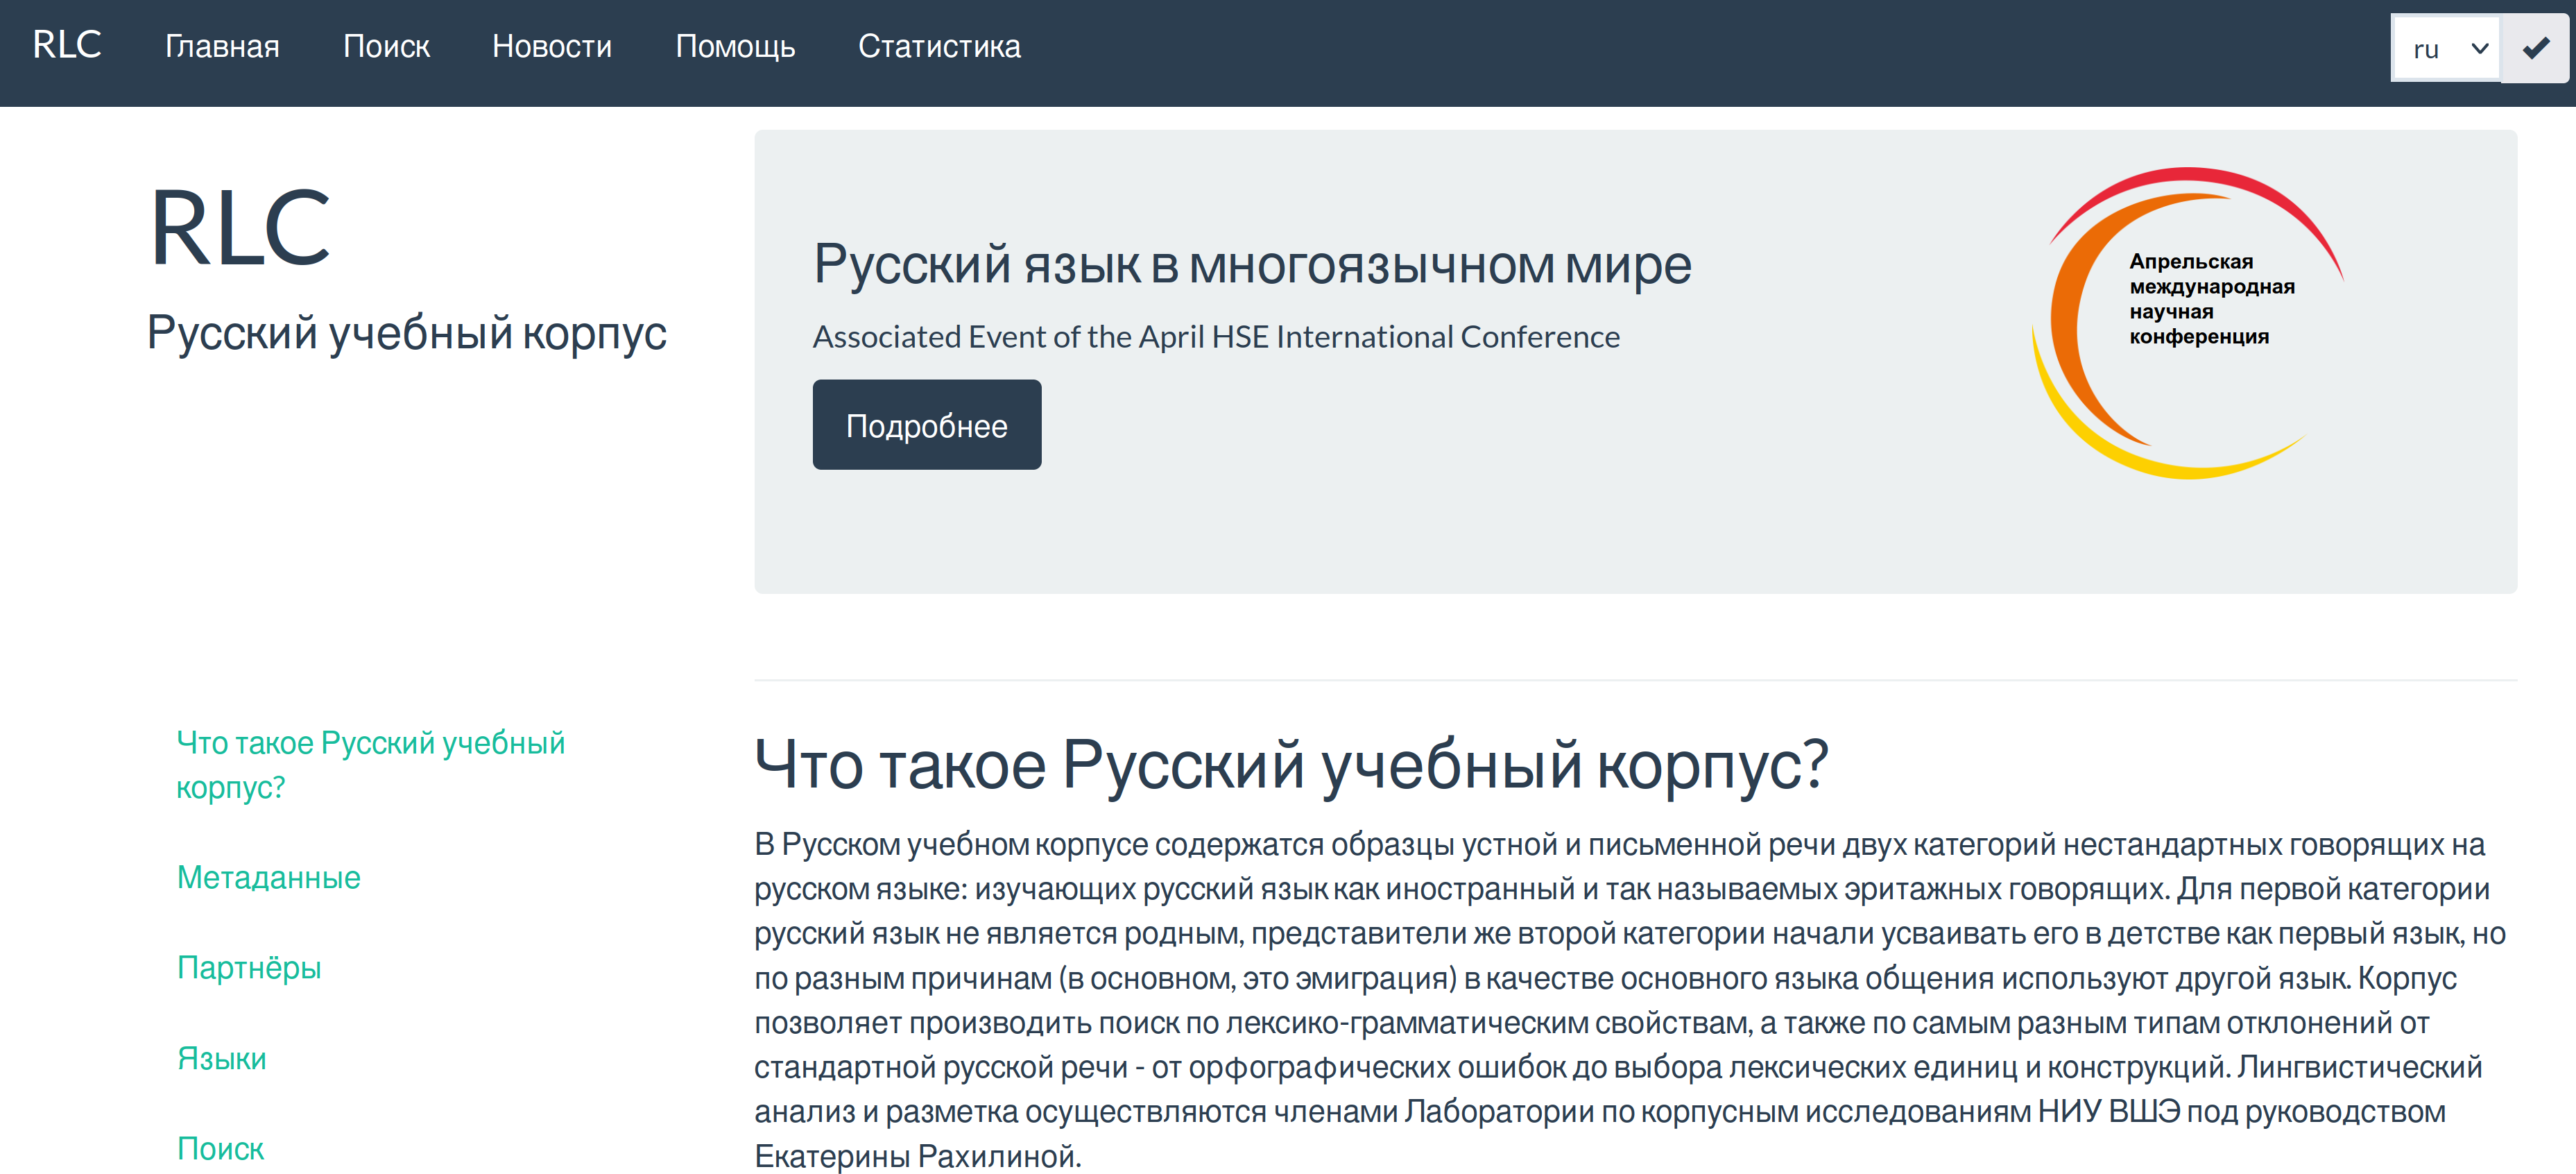
\includegraphics[width=0.98\linewidth]{images/RLC} \end{center}
\end{frame}

\begin{frame}{Создание тренажеров}
\protect\hypertarget{ux441ux43eux437ux434ux430ux43dux438ux435-ux442ux440ux435ux43dux430ux436ux435ux440ux43eux432}{}
\begin{itemize}
\tightlist
\item
  \url{https://agricolamz.github.io/language_of_science_website/}
\end{itemize}

\begin{center}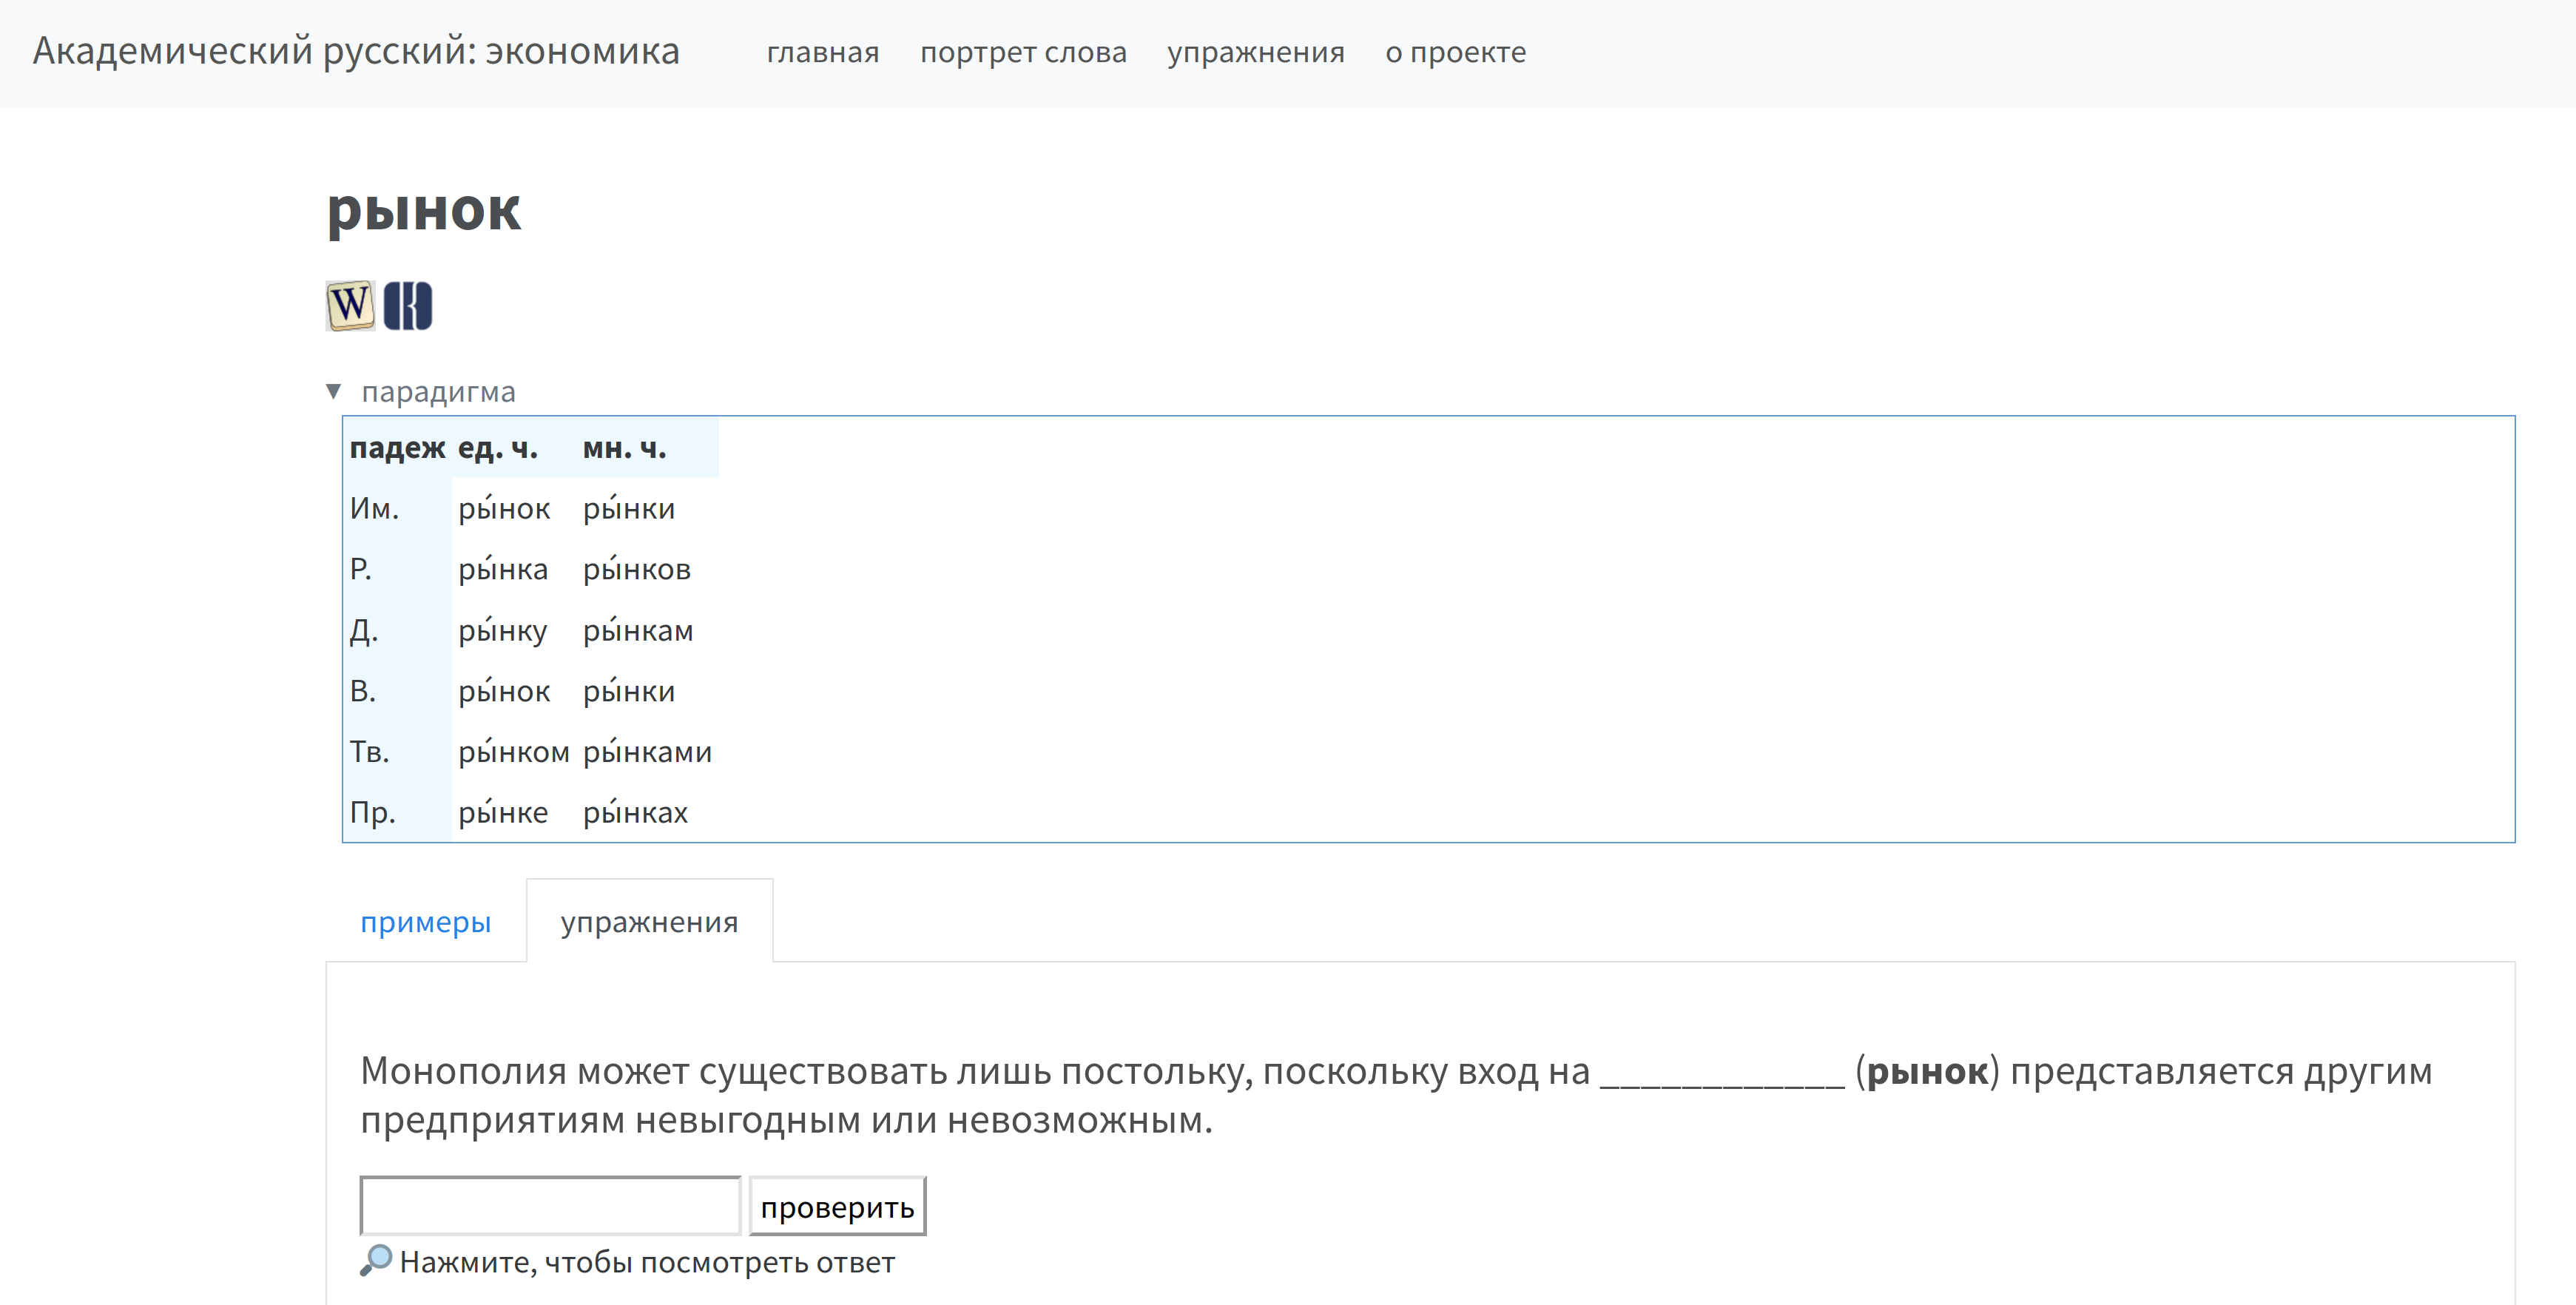
\includegraphics[width=0.98\linewidth]{images/economy} \end{center}
\end{frame}

\begin{frame}{Взаимодействие}
\protect\hypertarget{ux432ux437ux430ux438ux43cux43eux434ux435ux439ux441ux442ux432ux438ux435}{}
\begin{itemize}
\tightlist
\item
  активный обмен опытом
\item
  лекции сотрудников НИУ ВШЭ для студентов ЮФУ
\item
  совместная конференция по цифровым гуманитарным исследованиям в 2023
  году
\end{itemize}
\end{frame}

\hypertarget{ux43fux43eux442ux435ux43dux446ux438ux430ux43b-ux43dux438ux436ux43dux435ux432ux430ux440ux442ux43eux432ux441ux43aux43eux433ux43e-ux433ux43eux441ux443ux434ux430ux440ux441ux442ux432ux435ux43dux43dux43eux433ux43e-ux443ux43dux438ux432ux435ux440ux441ux438ux442ux435ux442ux430}{%
\section{Потенциал Нижневартовского государственного
университета}\label{ux43fux43eux442ux435ux43dux446ux438ux430ux43b-ux43dux438ux436ux43dux435ux432ux430ux440ux442ux43eux432ux441ux43aux43eux433ux43e-ux433ux43eux441ux443ux434ux430ux440ux441ux442ux432ux435ux43dux43dux43eux433ux43e-ux443ux43dux438ux432ux435ux440ux441ux438ux442ux435ux442ux430}}

\begin{frame}{Изучение хантыйского языка}
\protect\hypertarget{ux438ux437ux443ux447ux435ux43dux438ux435-ux445ux430ux43dux442ux44bux439ux441ux43aux43eux433ux43e-ux44fux437ux44bux43aux430}{}
\begin{itemize}
\tightlist
\item
  профиль «Хантыйская филология»
\item
  профиль «Искусственный интеллект в моделировании речевой деятельности»
\end{itemize}
\end{frame}

\begin{frame}{Хантыйский и мансийский языки}
\protect\hypertarget{ux445ux430ux43dux442ux44bux439ux441ux43aux438ux439-ux438-ux43cux430ux43dux441ux438ux439ux441ux43aux438ux439-ux44fux437ux44bux43aux438}{}
\begin{itemize}
\tightlist
\item
  Ob-Ugric database, Германия, Университет Людвига-Максимилиана, Мюнхен.
  Е. К. Скрибник
\item
  \url{https://www.babel.gwi.uni-muenchen.de/} \pause
\item
  ЛингвоДок, Россия, ИСП РАН, ИЯз РАН. Норманская Ю. В., Дыбо А. В.,
  Борисенко О.
\item
  \url{http://lingvodoc.ispras.ru/corpora_all?all=\&language=508\%2C44}
  \pause
\item
  NorthEuralex, Германия, Университет Тюбингена, Йоханнес Деллерт
\item
  \url{https://link.springer.com/article/10.1007/s10579-019-09480-6}
  \pause
\item
  UraTyp -- типологический ресурс из института Макса Планка
\item
  \url{https://uralic.clld.org/languages}
\end{itemize}
\end{frame}

\begin{frame}{}
\protect\hypertarget{section}{}
\LARGE Спасибо за внимание!
\end{frame}

\renewcommand\refname{Литература}
\begin{frame}[allowframebreaks]{Литература}
  \bibliographytrue
  \bibliography{bibliography.bib}
\end{frame}

\end{document}
